\documentclass[a4paper,onesided,12pt]{report}
\usepackage{styles/fbe_tez}
\usepackage[utf8x]{inputenc} % To use Unicode (e.g. Turkish) characters
\renewcommand{\labelenumi}{(\roman{enumi})}
\usepackage{amsmath, amsthm, amssymb}
 % Some extra symbols
\usepackage[bottom]{footmisc}
\usepackage{cite}
\usepackage{graphicx}
\usepackage{color}
\usepackage{booktabs}
\usepackage{longtable}
% \usepackage{caption}
% \usepackage{subfigure}
\usepackage{enumitem}
\usepackage{svg}
\usepackage{dirtree}
\usepackage{listings}
\lstset{
% numbers=right, 
% numberstyle=\small, 
% numbersep=8pt, 
frame = single, 
% language=Pascal, 
% framexleftmargin=15pt
}
%\usepackage[left=3.5cm, right=2cm, top=4cm, bottom=2cm]{geometry}
            
\graphicspath{{figures/}} % Graphics will be here

\usepackage{multirow}
\usepackage{subfigure}
\usepackage{algorithm}
\usepackage{algorithmic}
%\pagestyle{empty}
%\includeonly{introduction} % To only process the given file
%\usepackage{blindtext}
\newtheorem{thm}{Theorem}[chapter]
\newtheorem{prop}[thm]{Proposition}
\newtheorem{lem}[thm]{Lemma}
\newtheorem{cor}[thm]{Corollary}
% COVER PAGE
\title{EMPOWERING HETEROGENEOUS NETWORKS FOR DRUG-TARGET AFFINITY PREDICTION}
\turkcebaslik{\.{I}LA\c{C}-HEDEF BA\u{G}LILIK \.{I}LG\.{I}S\.{I} TAHM\.{I}N\.{I} \.{I}\c{C}\.{I}N HETEROJEN A\u{G}LARI G\"{U}\c{C}LEND\.{I}RME }
\degree{B.S., Computer Engineering, Marmara University, 2018}
\author{Selen Parlar}
\program{Computer Engineering}
\subyear{2022}

% APPROVED BY PAGE
\supervisor{Assoc. Prof. Arzucan \"{O}zg\"{u}r}
\cosuperi{Assoc. Prof. Elif \"{O}zk{\i}r{\i}ml{\i} \"{O}lmez}

\examineri{Prof. Tunga G\"{u}ng\"{o}r}

\examinerii{Prof. Nilg\"{u}n L\"{u}tfiye Karal{\i}\quad\quad\quad}
% \examineri{Name Surname, Ph.D.}
% \examineri{Name Surname, Ph.D.}
%\examineriv{}
%\examinerv{}
\dateofapproval{27.01.2022}



\begin{document}

\pagenumbering{roman}
\makemstitle 
\makeapprovalpage


\begin{acknowledgements}
First of all, I would like to thank my advisors: Assoc. Prof. Elif Özkırımlı for her support and patience during my studies and Assoc. Prof. Arzucan Özgür for her guidance, trust in me, and big heart that she has as an academic mom. Thank you for all the big hugs you gave virtually and personally. 

I want to express my gratitude to my jury members, Prof. Tunga Güngör and Prof. Nilgün Lütfiye Karalı, for kindly accepting to participate in the defense of this thesis and for all the comments and critics that improved my study. 

I gratefully acknowledge TÜBİTAK ARDEB 1001 Program (Project No: 119E133) and the TAM project for providing the computational resources. 

I also thank my lab-mates, whom I cannot list here since they are a lot, but I will always remember you in front of my window, full of flowers with the view of the North Campus pyramid. 

I am grateful to my family, Nuray Parlar and Mustafa Parlar, for always supporting me and giving me the opportunities that have made me who I am. Also, I would like to thank my chosen family, M.D. İremnaz Karahan and Mert Aydın for providing a mirror to my life. Last but not least,  my cat Fındık, which is like a child to me, thank you for opening a window to my heart. 

The completion of this study could not have been possible without the expertise, patience, love, support, and hugs of my dearest lifelong best friend, desk-mate, and love of my life, Rıza Özçelik. This thesis is dedicated to our new family, and I love you as much as the words in this thesis (23,235), believe it or count it.
\end{acknowledgements}
\begin{abstract}
One page abstract will come here.  
\end{abstract}
\begin{ozet}
Bir sayfa uzunluğunda özet gelecektir.
\end{ozet}
\tableofcontents
\listoffigures
\listoftables
\begin{symbols}
% The title will be typeset as "LIST OF SYMBOLS".
%
% Use a separate \sym command for each symbols definition.
% First, Latin symbols in alphabetical order
\sym{$a_{ij}$}{Description of $a_{ij}$}
\sym{$\mathbf{A}$}{State transition matrix of a hidden Markov model}
% 1 EMPTY LINE BETWEEN LATIN AND GREEK SYMBOLS GROUP!!!
\sym{}{}
% Then Greek symbols in alphabetical order
\sym{$\alpha$}{Blending parameter \textit{or} scale}
\sym{$\beta_t(i)$}{Backward variable}
\sym{$\Theta$}{Parameter set}
\sym{ }{}

\end{symbols}

\begin{abbreviations}
 % Abbreviations in alphabetical order
\sym{ADMET}{Chemical absorption, distribution, metabolism, excretion, and toxicity}
\sym{CID}{Compound ID Number}
\sym{CTD}{Comparative Toxicogenomics Database}
\sym{DOI}{Digital Object Identifier}
\sym{EC50}{The Concentration of Compound that Generates a Half-Maximal Response}
\sym{EMBL}{European Molecular Biology Laboratory}
\sym{IC50}{The Concentration of Ligand that Reduces Enzyme Activity by 50\%}
\sym{InChI}{International Chemical Identifier}
\sym{Kd}{Kinase Dissociation Constant}
\sym{Ki}{Kinase Inhibition Constant}
\sym{nM}{Nanometer}
\sym{pKd}{Log Transformed Dissociation Constant}
\sym{SMILES}{Simplified Molecular-Input Line-Entry System}
\sym{UniProt}{The Universal Protein Source}

\sym{1D}{One Dimensional}
\sym{2D}{Two Dimensional}
\sym{3D}{Three Dimensional}
\sym{100D}{One Hundred Dimensional}

\sym{BoW}{Bag of Words}
\sym{BPE}{Byte Pair Encoding}
\sym{CI}{Concordance Index}
\sym{DTA}{Drug-Target Affinity}
\sym{DTI}{Drug-Target Interaction}
\sym{LM}{Language Model}
\sym{MACCS}{Molecular Access System}
\sym{MSE}{Mean Squared Error}
\sym{MSS}{Maximum Sequence Similarity}
\sym{NLP}{Natural Language Processing}
\sym{OOV}{Out of Vocabulary}
\sym{RMSE}{Root Mean Squared Error}
\sym{SMILES}{Simplified Molecular Input Entry Specification}
\sym{SW}{Smith-Waterman}
\sym{ULM}{Unigram Language Model}
\end{abbreviations}

\chapter{INTRODUCTION}
\label{chapter:introduction}
\pagenumbering{arabic}
Drug design is an expensive and time-consuming process that can be carried out by testing the existing chemicals on different types of protein targets \cite{csermely2013structure}. Furthermore, drug design is a highly dynamic field due to the continuous evolution of target proteins and their different responses to the same drugs over time. During the process, several factors are considered such as protein-ligand binding affinity, bioactive conformation, pharmacokinetic parameters, metabolic stability, selectivity, toxicity, and synthesizability.

The main goal of drug design is to provide a selective effect while minimizing the side-effects by targeting only the disease-specific receptors and protecting the healthy cells. Today, rational designs that save time and cost in the pharmaceutical design are applied and it is possible to develop drugs with selectively effective and fewer side effects. This rational discovery process often begins with the development of a drug active substance, by selecting and improving ligands from a molecule library. However, the size of the drug search space is huge when we consider the existence of 97 million chemicals in the chemical database PubChem \cite{bolton2008pubchem} and the 16,526 drugs in the DrugBank \cite{law2013drugbank}. Due to the expansive search space, the need for computational methods has emerged for this multi-stage, trial and error based process. 

Computational methods aim to determine the interacting and non-interacting drug and target pairs, and binary classification methods have been commonly used \cite{yamanishi2010drug, liu2016neighborhood, nascimento2016multiple, keum2017self, greenside2017prediction}. Binary classification-based approaches provide information about a possible interaction between proteins and ligands, however, the strength of the protein-ligand interactions, namely the binding affinity, cannot be determined with these methods. Binding affinity is important  in the drug design pipeline since a strong interaction is the first step in finding a selective drug. However, prediction of the binding affinity value still remains a challenge \cite{ozturk2018deepdta}. In this thesis, we propose a graph-based model to predict the drug target binding affinities.
% Continue with the actual proposal

%Start with an introduction...
\chapter{RELATED WORK}
\label{related_work}

<<<<<<< Updated upstream
=======
<<<<<<< HEAD
The computational methods used in drug discovery recently focused on four strategies; ligand similarity-based \cite{keiser2007relating}, molecular docking/structure-based \cite{morris2009autodock4,donald2011algorithms}, deep learning-based \cite{wan2018neodti, luo2017network}, and network-based approaches \cite{luo2017network, zheng2013collaborative, chen2012drug, wang2014drug}. The performance of the ligand similarity-based approaches is often low when a target has a few known binding ligands. Also, the limited availability of 3D structures of target proteins limits the molecular docking performance. Due to the limited data availability, some efforts have been devoted to developing machine learning-based approaches for drug target affinity (DTA) predictions through computational techniques. The growing amount of drug-target binding affinity data available in online databases has led to the adoption of advanced learning techniques such as deep learning architectures in predicting binding affinities \cite{chan2016large, tian2016boosting, hamanaka2017cgbvs, ozccelik2021chemboost, ozturk2018deepdta, ozturk2019widedta}. Last but not least, with networks, the ability to integrate several types of information, the affinity prediction task gained some other insights, and in the last decade, the number of studies increased \cite{wan2018neodti, luo2017network, nguyen2019graphdta}.

%Protein-ligand scoring is used to approximately predict the binding affinity between two molecules, and it is frequently used after the virtual screening, and docking campaigns \cite{ragoza2017protein}. One of the successful alternative machine learning methods to scoring functions is the Random Forest algorithm \cite{ballester2010machine, shar2016pred}. However, it fails in virtual screening and docking tests due to oversimplification of the protein-ligand complex descriptions \cite{gabel2014beware}. The continuously expanding amount of protein-ligand binding data enables deep learning methods in scoring. For instance, 3D structures of protein-ligand complexes are commonly used with Convolutional Neural Networks (CNNs) \cite{gomes2017atomic, ragoza2017protein, wallach2015atomnet}; however, its success is limited to known protein-ligand complex structures. Kronecker Regularized Least Squares (KronRLS) algorithm is also used in scoring \cite{pahikkala2014toward}. Only 2D compound similarity-based drug representations and Smith-Waterman similarity representations of the targets are used in KronRLS. Another approach proposed to predict the binding affinity scores is SimBoost method \cite{he2017simboost}. It uses a gradient boosting machine with extracted features from drug-target pairs' interactions and similarity-based information. 

Several types of deep learning frameworks have been adopted in the DTA prediction task. DeepDTA \cite{ozturk2018deepdta} and WideDTA \cite{ozturk2019widedta} approaches are proposed to predict the binding affinities of protein-ligand interactions. Both methods utilize deep learning models that use only 1D representations of proteins and ligands. As the 1D representation, both studies use SMILES (Simplified Molecular Input Line Entry System) representations of the compounds rather than complex external features. DeepDTA learns high dimensional features from full-length sequences of the proteins and ligands. It uses two Convolutional Neural Networks (CNNs) to learn the representations of drugs and proteins. Then, the concatenated representations of drugs and proteins are fed into a multi-layer perceptron (MLP). 
Nevertheless, it fails to capture the biologically important short subsequences. WideDTA overcomes this problem by integrating different kinds of text-based information such as protein sequence, ligand SMILES, protein domains and motifs, and maximum common substructure words to provide better representation and predict binding affinity. To do that, WideDTA employs four CNNs and learns the representations of drugs and proteins. 
Similarly, it uses the MLP with the concatenated representations. The DeepConv-DTI \cite{lee2019deepconv} also utilizes CNNs on the protein sequences. On the other hand, they use 2D structural images of chemicals to learn complex features using CNNs and produce DTA predictions.

Although the extensive experiments and enhanced performance in the DTA prediction task, representing the drugs as strings cause a loss of information since 1D representations cannot fully represent the structural information beneath the biomolecules. Graph neural networks (GNNs) are employed to address this problem, and drugs are represented as graphs. Tsubaki \textit{et al.} \cite{tsubaki2019compound} propose to use CNNs and GNNs together to learn the representation of compound graphs and protein sequences. They demonstrate performance improvement on the DTA task compared to the feature-based methods. GraphDTA \cite{nguyen2019graphdta} also suggests a new neural network architecture for the drug-target affinity prediction task. Rather than using the 1D representation of SMILES, they convert SMILES representation into a molecular graph and employ a graph neural network (GNN) to learn a graph representation. Moreover, they encode and embed protein amino acid sequences and use CNN to create protein representations. Then, combine CNNs and GNNs to predict the binding affinity value. Another method, DGraphDTA \cite{jiang2020drug}, uses graphs to represent both compounds and proteins with GNNs. Additionally, to address the interpretability, several models employ an attention mechanism \cite{karimi2020explainable, chen2020transformercpi, agyemang2020multi, yang2021ml}. 

Rather than using only the known drug-target interaction (DTI) data in deep learning models, some other diverse information from heterogeneous data sources integrated into the systems, such as protein-protein interaction (PPI), drug-disease association, drug-side effect association as in the work of MSCMF \cite{zheng2013collaborative}, HNM \cite{wang2014drug}, DTINet \cite{luo2017network}, and NeoDTI \cite{wan2018neodti}. They employ networks that can capture the complex relationships between different types of components, such as drugs and proteins. These methods have improved the performance in the DTI prediction task, yet they have some limitations to be addressed. For instance, in MSCMF \cite{zheng2013collaborative}, drug and protein similarity matrices are gathered from different data sources via a weighted averaging scheme in order to use in the matrix factorization of a given DTI network. However, this data integration often causes data loss, resulting in a suboptimal solution. Moreover, DTINet \cite{luo2017network} is developed as a computational pipeline to predict novel DTI from a heterogeneous network. First, it learns low-dimensional feature representations of drugs and targets in an unsupervised manner. Then it predicts new DTIs with inductive matrix completion (IMC) as in the work of Natarajan and Dhillon \cite{natarajan2014inductive}. Since DTINet handles the unsupervised feature learning procedure and the prediction task separately, it may cause non-optimal solutions. NeoDTI \cite{wan2018neodti} targets this problem and combines feature learning and classification into a single task, improving the accuracy. 

More recently, Zhao \textit{et al.} \cite{zhao2021identifying} propose a method that combines GNNs and deep neural networks (DNNs) for the DTI prediction task. They build a drug-protein network using drug-drug interaction, protein-protein interaction, and drug-protein interaction networks in which nodes represent drugs and proteins, and edges represent the link strength between them. Then, handles the DTI prediction problem as a node classification problem. Another network-based method EEG-DTI \cite{peng2021end} proposes an end-to-end heterogeneous graph representation learning-based framework to predict the interaction between drugs and targets using graph convolutional networks (GCNs). DTiGEMS$+$ \cite{thafar2020dtigems+} constructs a heterogeneous graph using the DTI graph with drug-drug similarity and target-target similarity graphs. It combines feature-based and similarity-based approaches to model the identification of drug-target pairs. After performing graph augmentation, it applies node2vec \cite{grover2016node2vec} for feature representation learning of drugs and targets and uses them in a link prediction task. To improve the DTiGEMS$+$'s performance, DTi2Vec \cite{thafar2021dti2vec} is proposed in which representation learning and ensemble learning techniques are combined to identify the drug-target interactions. Unlike the previous work, it uses edge embeddings between drug-target node pairs rather than node embeddings. Given the success of heterogeneous graphs in the DTI prediction and text-based methods in DTA prediction, in this thesis, we propose a method for DTA prediction that utilizes heterogeneous graphs together with the biomolecular language-based information obtained from the text representations of chemicals and proteins. 
%This is the first study that combines heterogeneous graphs and biomolecular language-based information for the DTA prediction task to the best of our knowledge. 

% Yine biraz karisiklik var. Metotlari detayli anlatmissin. Emege saygi +rep. Ama genel cerceveden kopmak cok kolay oluyor okurken. Arada olaylari birbirine baglamak ve neyi neden anlattigina dair bir seyler yazmak iyi olabilir.

% Karisik pargraflari toplamak icin bkz: tek cumlelik ozet
=======
>>>>>>> Stashed changes
Traditional computational methods used in drug discovery are based on four strategies; ligand similarity-based \cite{keiser2007relating}, molecular docking/structure-based \cite{morris2009autodock4,donald2011algorithms}, deep learning-based \cite{wan2018neodti, luo2017network}, and network-based approaches \cite{luo2017network, zheng2013collaborative, chen2012drug, wang2014drug}. The performance of the ligand similarity-based approaches is often low when a target has a few known binding ligands. Likewise, the limited availability of 3D structures of target proteins limits the molecular docking performance. In the last decade, some effort has been devoted to developing machine learning-based approaches for drug target affinity (DTA) predictions through computational techniques. Binding affinity provides information on the strength of the interaction between a drug-target pair and the increase in available affinity data in online databases has led to the use of advanced learning techniques such as deep learning architectures in predicting binding affinities \cite{chan2016large, tian2016boosting, hamanaka2017cgbvs}.

Protein-ligand scoring is used to approximately predict the binding affinity between two molecules, and it is frequently used after virtual screening and docking campaigns \cite{ragoza2017protein}. One of the successful alternative machine learning methods to scoring functions is Random Forest algorithm \cite{ballester2010machine, shar2016pred}. However, it fails in virtual screening and docking tests due to oversimplification of the protein-ligand complex descriptions \cite{gabel2014beware}. The continuously expanding amount of protein-ligand binding data enables the use of deep learning methods in scoring. For instance, 3D structures of protein-ligand complexes are commonly used with Convolutional Neural Networks (CNNs) \cite{gomes2017atomic, ragoza2017protein, wallach2015atomnet}, however, its success is limited to known protein-ligand complex structures. Kronecker Regularized Least Squares (KronRLS) algorithm is also used in scoring \cite{pahikkala2014toward}. It utilizes only 2D based compound similarity-based representations of the drugs and Smith-Waterman similarity representation of the targets. Another approach proposed to predict the binding affinity scores is SimBoost method \cite{he2017simboost}. It uses a gradient boosting machine with the extracted features from interactions between drug-target pairs and their similarity-based information. 

Several types of deep learning frameworks have been adopted in DTA prediction task. DeepDTA \cite{ozturk2018deepdta} and WideDTA \cite{ozturk2019widedta} approaches are proposed to predict the binding affinities of protein-ligand interactions. Both methods utilize deep learning models that use only 1D representations of proteins and ligands. As the 1D representation, both of the studies use SMILES (Simplified Molecular Input Line Entry System) representations of the compounds rather than complex external features or 3D-structures of the binding complexes. DeepDTA learns high dimensional features from full-length sequences of the proteins and ligands. It uses two CNNs to learn the representations of drugs and proteins. Then, the concatenated representations of drugs and proteins are fed into the a multi-layer perceptron (MLP). Yet, it fails to capture the biologically important short subsequences. WideDTA overcomes this problem by integrating different kinds of text-based information such as protein sequence, ligand SMILES, protein domains and motifs, and maximum common substructure words to provide better representation and to predict binding affinity. To do that, WideDTA employs four CNNs and learn the representations of drugs and proteins. Similarly, uses the MLP with the concatenated representations. Lee \textit{et al.} \cite{lee2019deepconv} also utilizes CNNs on the protein sequences. On the other hand, they use 2D structural images of chemicals and learn complex features from them using CNNs and produce DTA predictions.

Although the extensive experiments and remarkable performance in DTA prediction task, representing the drugs as strings cause loss of information due to structural information lies beneath the molecules. To address this problem, graph neural networks (GNNs) are employed and drugs are represented as graphs. Tsubaki \textit{et al.} \cite{tsubaki2019compound} propose to use CNNs and GNNs together to learn the representation of compound graphs and protein sequences. They demonstrate performance improvement on DTA task compared to the feature-based methods. GraphDTA \cite{nguyen2019graphdta} also suggests a new neural network architecture for drug-target affinity prediction task. Rather than using the 1D representation of SMILES, they convert SMILES representation into a molecular graph and employ a graph neural network (GNN) to learn a graph representation. Moreover, they encode and embed protein amino acid sequences and use CNN to create protein representations. Then, combine CNNs and GNNs to predict the binding affinity value. Another method, DGraphDTA \cite{jiang2020drug}, uses graphs to represent both compounds and proteins and with GNNs. Additionally, to address the interpretability, several models employ attention mechanism \cite{karimi2020explainable, chen2020transformercpi, agyemang2020multi, yang2021ml}. 

Rather than using only the known drug-target interaction (DTI) data in deep learning models, some other diverse information from heterogeneous data sources integrated into the systems, such as protein-protein interaction (PPI), drug-disease association, drug-side effect association as in the work of MSCMF \cite{zheng2013collaborative}, HNM \cite{wang2014drug}, DTINet \cite{luo2017network}, and NeoDTI \cite{wan2018neodti}. They employ networks that are able to capture the complex relation between different types of components such as drugs and proteins. These methods have improved the performance in DTI prediction task, yet they have some limitations to be addressed. In MSCMF \cite{zheng2013collaborative}, drug and protein similarity matrices are gathered from different data sources via a weighted averaging scheme in order to use in matrix factorization of a given DTI network. However, this data integration often causes data loss that will result in a suboptimal solution. DTINet \cite{luo2017network} is developed as a computational pipeline to predict novel DTI from a heterogeneous network. First, it learns low-dimensional feature representations of drugs and targets with an unsupervised manner, then it predicts new DTIs with inductive matrix completion (IMC) as in the work of Natarajan and Dhillon \cite{natarajan2014inductive}. Since DTINet handles the unsupervised feature learning procedure and the prediction task separately, it may cause non-optimal solutions. NeoDTI \cite{wan2018neodti} targets this problem and combines feature learning and classification into a single task, improving the accuracy. 

More recently, Zhao \textit{et al.} \cite{zhao2021identifying} propose a method that combines GNNs and deep neural networks (DNNs) for DTI prediction task. They build a drug-protein network using drug-drug interaction, protein-protein interaction, and drug-protein interaction networks in which a nodes represent drug and proteins and edges represent the link strength between them. Then, handle the DTI prediction problem as a node classification problem. Another network-based method EEG-DTI \cite{peng2021end} proposes an end-to-end heterogeneous graph representation learning-based framework to predict the interaction between drugs and targets using graph convolutional networks (GCNs). DTiGEMS$+$ \cite{thafar2020dtigems+} constructs a heterogeneous graph using the DTI graph with drug-drug similarity and target-target similarity graphs. It combines feature-based and similarity-based approaches to model the identification of drug-target pairs. After performing graph augmentation, it applies node2vec \cite{grover2016node2vec} for feature representation learning of drugs and targets and use them in a link prediction task. To improve the DTiGEMS$+$'s performance, DTi2Vec \cite{thafar2021dti2vec} is proposed in which representation learning and ensemble learning techniques are combined to identify the drug-target interactions. Unlike the previous work, it uses edge embeddings between drug-target node pair rather than the node embeddings.

<<<<<<< Updated upstream
Given the success of heterogeneous graphs in DTI prediction and text-based methods in DTA prediction, in this thesis we propose a method for DTA prediction that utilizes heterogeneous graphs. Moreover, in order to enrich the heterogeneity of the graph, we propose to add biomolecular language-based information obtained from the 1D structure. To the best of our knowledge, this is the first study that combines heterogeneous graphs and biomolecular language-based information for the DTA prediction task. 
=======
Given the success of heterogeneous graphs in DTI prediction and text-based methods in DTA prediction, in this thesis we propose a method for DTA prediction that utilizes heterogeneous graphs. Moreover, in order to enrich the heterogeneity of the graph, we propose to add biomolecular language-based information obtained from the 1D structure. To the best of our knowledge, this is the first study that combines heterogeneous graphs and biomolecular language-based information for the DTA prediction task. 
>>>>>>> d09ebba9e602d1522ef9361417dc21d129009597
>>>>>>> Stashed changes

\chapter{BACKGROUND}
\label{background}

\section{Graphs}
A graph $G = (V, \varepsilon)$ is defined by a set of nodes $V$ and a set of edges $E$ between these nodes as going from node $u \in V$ to node $v \in V$ as $(u,v) \in \varepsilon$. In this thesis, we concern only simple graphs, i.e., there exists at most one edge between each pair of nodes, and no edges between  a node and itself. Moreover, all edges are undirected, so $(u,v) \in \varepsilon \longleftrightarrow (u,v) \in \varepsilon$. A graph has a single type of edge or different type of edges. In a multi-relational graph the edge notation can be extended as $(u,\tau,v) \in \varepsilon$ to include the relation type $\tau$ \cite{hamilton2020graph}. Throughout the thesis we consider two important subsets of graphs; homogeneous and heterogeneous i.e., graphs with single and multiple relation types respectively. 

Graph is homogeneous when all the nodes represents the instances of the same type and all the edges represents the same type of relations. For instance, drug-drug interaction network is a homogeneous graph consisting of drugs and the connections between drugs, representing the same type of entity. Figure \ref{fig:sample_ddi} shows a homogeneous drug-drug interaction graph with five drugs, and the risk or severity of bleeding can be increased when Cyclosporine is combined with Phenylalanine \cite{ihlefeldt2014polymorphs}. 

\begin{figure}
    \centering
        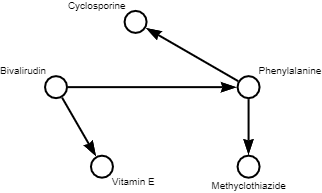
\includegraphics[width=0.5\linewidth]{chapters/background/figures/ddi.png} 
    \caption{Homogeneous Drug-Drug Interaction Graph.}
    \label{fig:sample_ddi}
\end{figure}

Graph is heterogeneous if the set of nodes can be partitioned into disjoint sets $V = V_{1} \cup V_{2} \cup ... \cup V_{k} $ where $V_{i} \cap V_{j} = \emptyset , \forall i \neq j$ \cite{sun2013mining}. For instance, drug-disease network is a heterogeneous graph consisting of two types of nodes as drugs and diseases, and two types of edges representing the \textit{treatment} relation that occurs only between drug nodes and disease nodes, and similarly \textit{polypharmacy side effect} that occurs only between two drug nodes. Figure \ref{fig:sample_ddi} shows a heterogeneous drug-disease association graph with 4 drugs, three disease, and two types of edges. For instance, the risk or severity of neutropenia can be increased when Methyclothiazide is combined with Phenylalanine \cite{ruiz2022primary}. 

\begin{figure}
    \centering
        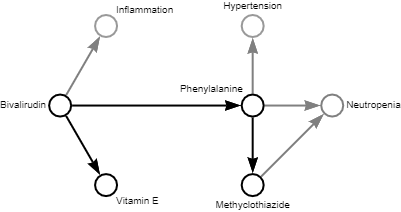
\includegraphics[width=0.65\linewidth]{chapters/background/figures/dda.png} 
    \caption{Heterogeneous Drug-Disease Association Graph.}
    \label{fig:sample_dda}
\end{figure}


\section{Graph Representation Learning}
The rapid development of molecular biology, bioinformatics, and cheminformatics and the increase in the number of available data have led the modeling the biological components as nodes and the interactions between nodes as edges of graphs. In the case of the drug discovery and disease treatment, it is crucial to examine the interactions between drug-drug, drug-disease, drug-protein, and protein-disease \cite{daminelli2012drug, davis2009comparative}. These interactions can be formed as heterogeneous graphs and used in knowledge extraction. Traditional machine learning algorithms use the data represented in Euclidean domain such as 1D sequences of proteins, 2D biomedical image, or 3D protein structure. However, graphs form a non-Euclidean domain and create a challenge due to its complex topological structure, diverse node connections, and arbitrary neighbor size. To address these challenges, graph representation learning is employed. Graph representation learning or graph embedding learns the low-dimensional representations of node or edges that can be used in downstream graph analytics or machine learning tasks such as node classification, and link prediction.

We use graph-based distributional representation learning method to represent the molecules. In general, this set of methods represents data that cannot be expressed in Euclidean space as a graph, and it aims to learn distributed vectors that reflect the semantic connections in the graph for nodes, edges or underlines in this graph \cite{wu2019comprehensive}. One of the most important advantages of this approach is that it can express the relationships between different types of nodes. Using the compiled data (See details in Chapter \ref{chapter:dataset_preparation}) we model protein, ligand, disease and side effect information and the extracted language-based information as different node types in a graph. The relationship between each node corresponds to different relationships such as protein-drug interaction and protein-protein interaction in our graph. By using the heterogeneous graph structure that we have obtained in this way, we learn the graph-based representation vectors for proteins and chemicals. In this heterogeneous graph, when distributional representations for chemicals and proteins are learned, the relationships of nodes with different concepts such as disease and side effects are also included in the representations. In this way, the output of the received vectors becomes richer in terms of information. 

To learn the distributional representation vectors we use MetaPath2Vec \cite{dong2017metapath2vec, pal2016deep}, which is a framework to learn representations of heterogeneous graphs. It is a neural network model that is designed to capture the rich semantics embedded in heterogeneous graphs by exploiting different types of relationships and meta-paths among nodes. To generate meaningful representations, it considers different semantics of relations, i.e., different meta-paths which are the sequence of node/edge types that denote relationships between node pairs.

MetaPath2Vec formalizes the representation learning problem in heterogeneous networks by leveraging the definitions in \cite{dong2017metapath2vec, sun2013pathselclus} as follows:

A heterogeneous network is a graph $G = (V, E, T)$ in which node $v$ is associated with edge $e$ with mapping functions $\phi(v) : V \to T_{V}$ and $\varphi(e) : E \to T_{E}$, respectively. The aim of heterogeneous network representation learning is to learn the d-dimensional representation $X \in R^{|V|\times d}, d \ll |V|$ , given a heterogeneous network $G$, that is able to capture the topological and semantic relations among them. Therefore, the resulting representation is low-dimensional matrix $X$, with the $v^{th}$  row corresponding to the representation of node $v$. Regardless of the node types in $V$, representations of each node are mapped into the same latent space. 

The word2vec model is proposed to learn the distributed representations of words within a corpus \cite{mikolov2013efficient, mikolov2013distributed}. Thereafter, DeepWalk \cite{perozzi2014deepwalk} and node2vec \cite{grover2016node2vec} models proposed, aiming to map the word-context concept of word2vec model into a network. DeepWalk and node2vec models use random walks to map the word-context concept and utilize the skip-gram model to learn the node representation in a homogeneous network. Their objective is to maximize the network probability \cite{mikolov2013distributed, perozzi2014deepwalk, grover2016node2vec}, that is:
\begin{equation}
    arg \max_{\theta} \prod_{v \in V}^{} \prod_{c \in N(V)}^{} p(c|v;\theta)
\end{equation}

where $N(v)$ denotes the node $v$'s neighborhood, in which $v$'s one-hop neighbors, and $p(c|v;\theta)$ defines the conditional probability of a context node $c$ given node $v$.

In the same way, metapath2vec introduces the heterogeneous skip-gram model for heterogeneous networks to model the heterogeneous neighborhood of a node. Therefore, metapath2vec aims to maximize the probability of having the heterogeneous context $N_{t}(v), t \in T_{V}$ given a node $v$:

\begin{equation}
    arg \max_{\theta} \sum_{v \in V}^{} \sum_{t \in T_{V} }^{} \sum_{c_{t} \in N_{t}(V)}^{} p(c_{t}|v;\theta)
\label{eq:context}
\end{equation}

where $N_{t}(v)$ denotes the node $v$'s neighborhood with the $t^{th}$ type of nodes. The $p(c_{t}|v;\theta)$ is a softmax function \cite{bengio2013representation, mikolov2013distributed}, that is:

\begin{equation}
    p(c_{t}|v;\theta) = \frac{e^{X_{c_{t}}}.X_{v}}{\sum_{u \in V}^{} e^{X_{u}}.X_{v}}
\label{eq:softmax}
\end{equation}

where $X_{v}$ is the $v^{th}$ row of $X$, corresponding to the embedding vector for node $v$. Mikolov \textit{et al.} also introduce negative sampling \cite{mikolov2013distributed} for optimization. With negative sampling, a small set of words are sampled from the corpus to construct the softmax. Same technique is also applied for metapath2vec, and Equation \ref{eq:context} is updated as follows:

\begin{equation}
    log\sigma(X_{c_{t}}.X_{v}) + \sum_{m=1}^{M} \mathbb{E}_{u^{m}\sim P(u)}[log\sigma(-X_{u^{m}}.X_{v})]
\end{equation}

where $M$ is the negative sample size, $\sigma (x) = \frac{1}{1+e^{-x}}$ and $P(u)$ is the pre-defined distribution in which node $u^{m}$ is drew from $M$ times.

In order to transform heterogeneous network structures into metapath2vec's skip-gram, that design a meta-path-based random walks, and generate paths. A meta-path schema is a path, denoted as $V_{1} \xrightarrow[]{R_{1}} V_{2} \xrightarrow[]{R_{2}}\cdots V_{t} \xrightarrow[]{R_{t}} V_{t+1} \cdots \xrightarrow[]{R_{l-1}} V_{l}$, where $R = R_{1} \circ R_{2} \circ \cdots \circ R_{l-1}$ defines the composite relations between node types $V_{1}$ and $V_{l}$ \cite{sun2012mining}.

As shown above, metapath2vec uses random walks guided by meta-paths to generate heterogeneous node sequences that are rich in semantics and structural information, then it designs a heterogeneous skip-gram model to preserve the node $v$'s proximity to its neighborhood nodes. It uses Equation \ref{eq:softmax} to calculate the similarity a node and its neighbors.

Based on metapath2vec, several variants have been proposed. For instance, BHIN2vec \cite{lee2019bhin2vec} proposes an extension to the skip-gram technique in order to balance the influence different relation types on node embeddings. HHNE \cite{wang2019hyperbolic} performs random walks in hyperbolic spaces. Another method, Hin2vec \cite{fu2017hin2vec}, combines first-order and high-order relations to capture the heterogeneity of graph and carries out multiple relation prediction tasks to jointly learn the node embeddings. In this thesis we employ metapath2vec since it is simpler and convenient to apply to large heterogeneous graph. Moreover, its code is open, so it is freely available to use and easy to adapt.\footnote{Code available at: https://github.com/apple2373/metapath2vec}

\section{Language-Based Representation Vector Learning}

\section{Affinity Prediction}

\section{Evaluation}
\chapter{MATERIALS AND METHODS}
This thesis predicts the binding affinity score of drug-target pairs by using heterogeneous graphs generated with the existing information and the language-based information extracted from chemical and protein sequences. We divided the study into five stages to do so, and this chapter summarizes these stages. In Stage 1, we compiled data from several online databases; in Stage 2, we assembled the compiled data and extracted useful information from them. In Stage 3, we created homogeneous and heterogeneous graphs using assembled data. Then in Stage 4, we learned the distributed vector representations of proteins and ligands using homogeneous and heterogeneous graphs with and without several language models. Finally, in Stage 5, we predict the affinity scores of drug-target pairs and evaluate the performance of our model using the evaluation metrics explained in Section \ref{section:evaluation}. 

\section{Dataset Compilation}
<<<<<<< Updated upstream
For the chemicals, we employ six databases and extract drug-related information such as unique IDs (InChI, CID, and DrugBank ID), SMILES strings, interacting drugs, interacting targets, side effects, and diseases. For the proteins, we used four databases and extract protein-related information such as unique IDs (Entrez Gene ID, and UniProt ID), amino acid sequences, interacting proteins, interacting drugs, and diseases. Figure \ref{fig:databases} shows these eight databases with the corresponding extracted information. 
=======
<<<<<<< HEAD
\label{section:dataset_compilation}
For the chemicals, we employ six databases and extract drug-related information; unique IDs (CID and DrugBank ID), SMILES strings, interacting drugs, interacting targets, side effects, and diseases. For the proteins, we use four databases and extracted protein-related information; unique IDs (Entrez Gene ID and UniProt ID), amino acid sequences, interacting proteins, interacting drugs, and diseases. 

Figure \ref{fig:databases} shows these eight databases with the corresponding extracted information. This section provides details and up-to-date statistical data about eight databases, namely BindingDB, ChEMBL, CTD, DrugBank, PubChem, SIDER, STRING, and UniProt.
=======
For the chemicals, we employ six databases and extract drug-related information such as unique IDs (InChI, CID, and DrugBank ID), SMILES strings, interacting drugs, interacting targets, side effects, and diseases. For the proteins, we used four databases and extract protein-related information such as unique IDs (Entrez Gene ID, and UniProt ID), amino acid sequences, interacting proteins, interacting drugs, and diseases. Figure \ref{fig:databases} shows these eight databases with the corresponding extracted information. 
>>>>>>> d09ebba9e602d1522ef9361417dc21d129009597
>>>>>>> Stashed changes

\begin{figure}
    \centering
        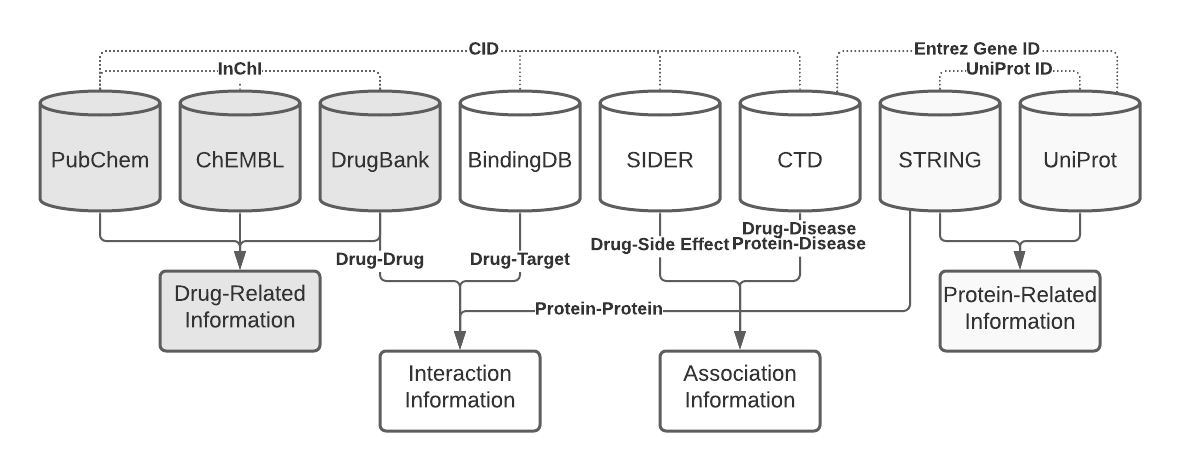
\includegraphics[width=\linewidth]{chapters/materials_and_methods/figures/databases.png}
    \caption{Compiled databases.}
    \label{fig:databases}
\end{figure}

<<<<<<< Updated upstream
=======
<<<<<<< HEAD
\newpage
\subsection{BindingDB}
BindingDB \cite{gilson2016bindingdb} is an online database of drug-target interactions and measured binding affinity values. As of February 2021, BindingDB contains 41,328 entries with DOI, 2,114,159 binding affinity data for 928,022 small molecules, and 8,202 protein targets. Binding affinity is usually expressed in measures such as inhibition constant ($K_i$), dissociation constant ($K_d$), and the half-maximal inhibitory concentration (IC50). For that purpose, 2,077,458 $K_i$ (nM), $K_d$ (nM), and IC50 (nM) values were compiled from the database within the scope of the thesis. 

To benchmark the performance of graph-based representational learning, we use BDB dataset \cite{ozccelik2021chemboost} that is filtered from the BindingDB database. 24,404 binding affinities were observed for all pairs of 924 ligand and 480 proteins, measured by the $pK_d$ value (log-transformed kinase dissociation constant) \cite{ozccelik2021chemboost}. $pK_d$ correlates positively with the binding strength, and the value varies between 1.6 and 13.3. The number of ligands with strong binding affinity values is 3,428 (\textit{i.e.}, $pK_d \geq 7$) according to literature \cite{he2017simboost}. Figure \ref{fig:bdb} illustrates the distribution of the binding affinity values of proteins - ligand pairs in the BDB dataset. 
\begin{figure}
    \centering
        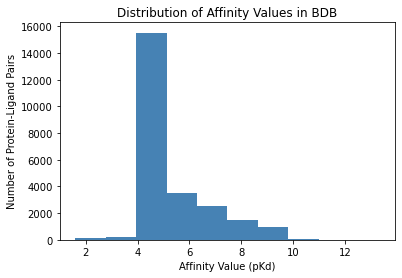
\includegraphics[width=0.5\linewidth]{chapters/materials_and_methods/datasetpreparation/figures/bdb.png} 
    \caption{Distribution of binding affinity values in BDB.}
    \label{fig:bdb}
\end{figure}

%BDB dataset consists of 5 different setups for training and evaluating the model performance. To evaluate the performance of DeepDTA, we trained the DeepDTA model with the knowledge derived from heterogeneous networks on five training setups of BDB dataset \cite{ozccelik2021chemboost}, and tested the models in the corresponding test sets. 
\subsection{ChEMBL}
ChEMBL \cite{davies2015chembl, gaulton2017chembl} is a manually curated chemical database of molecules with drug-like properties and biological activity, which is maintained by the European Molecular Biology Laboratory (EMBL). The ChEMBL database contains bioactivity data of active pharmaceutical ingredients, which are reported with $K_i$, $K_d$, and IC50 values. ChEMBL examines how small molecules interact with target proteins and how these compounds affect cells and whole organisms. Moreover, ChEMBL includes information about the 2D structure, calculated molecular properties, and the ADMET properties such as in vivo absorption, distribution, metabolism, excretion, and toxicity of small molecules. As of May 2020, there are 1,941,412 chemicals in the ChEMBL database and we extract 10,935 drugs' 1D text representations, \textit{i.e.,} SMILES strings from ChEMBL. Using SMILES strings of drugs, we trained the CNN-based model that encodes each SMILES string character as numbers and the language-based model that leverages the similarity between drugs' SMILES strings.
\subsection{Comparative Toxicogenomics Database}
The Comparative Toxicogenomics Database \cite{davis2021comparative} (CTD), is a database that provides information on manually curated chemical–gene$/$protein interactions, chemical-disease, and gene-disease relationships. CTD has several categories of data. These are chemicals, diseases, chemical-disease relationships, and gene-disease relationships. 

\begin{table}[ht]
\caption{CTD statistics (02.2021).}
\vspace{0.25em}
\centering
\begin{tabular}{|l|l|}
\hline
\multicolumn{1}{|c|}{\textbf{Data}} & \multicolumn{1}{c|}{\textbf{Number}} \\ \hline
Chemicals                  & 16,572                      \\ \hline
Diseases                   & 7,246                       \\ \hline
Chemical-Disease Relation  & 2,958,797                   \\ \hline
Gene-Disease Relation      & 28,253,189                  \\ \hline
\end{tabular}
\label{tab:ctd_stats}
\end{table}

Table \ref{tab:ctd_stats} shows the available number of chemicals, diseases, and the association between diseases and chemicals$/$genes, as of February 2021. Since some diseases are common for both chemicals and genes, we extracted 2,958,797 chemical-disease relationships and 28,253,189 gene-disease relationships within the scope of this thesis in order to generate heterogeneous graphs.


\subsection{DrugBank}
DrugBank \cite{wishart2006drugbank, wishart2008drugbank, wishart2018drugbank} is an online database that contains drugs, drug-related data (chemical, pharmacological, and pharmaceutical), and target-related data (sequence, structure, and pathway) as both bioinformatics and cheminformatics sources. As of January 2021, DrugBank contains 14,350 drugs. In the scope of this thesis, we extract 2,682,158 drug-drug interaction information of 14,350 drugs. We create homogeneous and heterogeneous graphs and generate representations for ligands using drugs and the relation between drugs.

% \begin{table}[]
\caption{DrugBank statistics (01.2021).}
\centering
\begin{tabular}{|l|l|}
\hline
\multicolumn{1}{|c|}{\textbf{Data}}  & \multicolumn{1}{c|}{\textbf{Number}} \\ \hline
Total Number of Small Molecule Drugs & 11.834                               \\ \hline
Total Number of Biotech Drugs        & 2.481                                \\ \hline
Total Number of Drugs                & 14.315                               \\ \hline
\end{tabular}
\label{tab:drugbank_stats}
\end{table}

\subsection{PubChem}
PubChem \cite{kim2021pubchem} is an online chemistry database that contains small molecules, nucleotides, as well as information on chemical structures, identifiers, chemical and physical properties. As of February 2021, the current statistics in the database are shown in Table \ref{tab:pubchem_stats}. 

\begin{table}[h]
\caption{PubChem statistics (02.2021)}
\vspace{0.25em}
\centering
\begin{tabular}{|l|l|}
\hline
\multicolumn{1}{|c|}{\textbf{Data}} & \multicolumn{1}{c|}{\textbf{Number}} \\ \hline
Compounds                           & 109,487,163                          \\ \hline
Substances                          & 270,034,522                          \\ \hline
Proteins                            & 96,280                               \\ \hline
Genes                               & 89,655                               \\ \hline
\end{tabular}
\label{tab:pubchem_stats}
\end{table}
\newpage
Since PubChem contains a considerable amount of data, other chemical databases map their entries with PubChem's Compound ID number (CID). In the context of this thesis, we leverage the PubChem CID of each chemical and map with the entries of BindingDB, SIDER, and CTD. Moreover, PubChem contains the International Chemical Identifier (InChI) of chemicals that textually identifies chemical substances. Similar to CID, We used chemicals' InChIs to relate the same chemicals across other databases, ChEMBL and DrugBank, that do not share any common IDs.
\subsection{SIDER}
SIDER \cite{kuhn2010side, kuhn2016sider} is a database of drugs that have entered the market and their recorded adverse drug reactions extracted from public documents and prospectuses. Side effect frequency, drug classification, side effect classification, and drug-target relationships are presented in a computer-readable format. SIDER uses the Anatomical Therapeutic Chemical (ATC) Classification System, a drug classification system that classifies the active substances of drugs according to the organ or system they act on and their therapeutic, pharmacological, and chemical properties. The Medical Dictionary codes side effects for Regulatory Activities (MedDRA) terminology, a clinically validated medical terminology thesaurus. The statistics as of October 2015 are shown in Table \ref{tab:sider_stats}. We used 5,868 side effects and extracted 139,756 drug-side effect relations.
\begin{table}
\caption{SIDER statistics (10.2015).}
\vspace{0.25em}
\centering
\begin{tabular}{|l|l|l|}
\hline
\textbf{Side Effects} & \textbf{Drugs} & \textbf{Drug-Side Effect Pairs} \\ \hline
5,868        & 1,430 & 139,756 \\ \hline
\end{tabular}
\label{tab:sider_stats}
\end{table}

\subsection{STRING}
Search Tool for the Retrieval of Interacting Genes$/$Proteins, STRING \cite{szklarczyk2021string}, is a biological database of known and predicted protein-protein interactions. The interactions include direct (physical) and indirect (functional) associations; they stem from computational prediction, from knowledge transfer between organisms, and interactions aggregated from other (primary) databases.

The STRING database compiles information from several sources such as computational prediction methods, public text collections, laboratory experiments, and other databases. According to the statistics provided as of August 2021, the STRING database contains 67,592,464 proteins and 296,567,750 interactions at the highest security (score $\geq$ 0.900), 834,790,438 interactions with high security or better (score $\geq$ 0.700), medium security or better 3,112,520,562 interactions (score $\geq$ 0.400), and a total of 20,052,394,041 interactions. We leverage the protein-protein interaction data and create a homogeneous database to learn the representations for proteins.
\subsection{UniProt}
The Universal Protein Source (UniProt) \cite{uniprot2021uniprot} is an essential resource for available protein information, including protein sequence and functional information. According to current statistics, as of September 2021, the total number of sequence entries is 565,928. Using amino acid sequences of proteins, we trained the CNN-based model that encodes each amino acid sequence character as numbers and the language-based model that leverages the similarity between proteins' amino acid sequences.


\section{Data Assembling}
\label{section:data_assembling}
This thesis aims to represent chemicals and proteins better. Therefore, chemical and protein-related data from several online databases are compiled. However, this task is not straightforward because of the vast amount of available data and the difficulty of standard mapping information across the databases. Therefore, we analyze the available data in the databases mentioned in Section \ref{section:dataset_compilation} and map the related information using common identifiers or unique sequences. Figure \ref{fig:databases} shows used databases as well as the IDs used to map corresponding databases.

\subsection{Chemical Related Information}
DrugBank, PubChem, and ChEMBL databases are the primary chemical resources, and we mainly focus on them. We compile 14,350 drugs from DrugBank and retrieve their DrugBank IDs and International Chemical Identifiers (InChI) as an initial step. Using InChIs, we connect the data in DrugBank with PubChem and ChEMBL databases and retrieve information about 10,935 different drugs. With 10,935 drugs, we extract 2,196,820 drug-drug relation information from the DrugBank database. Using the PubChem Compound ID number (CID) information available in the PubChem database, we map the PubChem to SIDER and CTD databases. We extract 5,452 distinct side effects from the SIDER database and 115,871 drug-side effect association information for 1,003 drugs. We extract 7,086 distinct diseases from the CTD database and 995,654 drug-disease association information for 3,387 drugs. Finally, we map DrugBank to ChEMBL and compile SMILES representations of 10,935 drugs using the InChI keys. 

Apart from the already existing information, we create a new relation named drug-drug similarity (DDS). Using the compiled SMILES representations of drugs from the ChEMBL database, DDS data is obtained by calculating the similarity of these representations to each other according to the Jaccard Similarity. In order to find similar SMILES sequences, we use the Byte Pair Encoding (BPE) algorithm \cite{sennrich2015neural}. The BPE approach is utilized to identify the language unit vocabulary of chemicals. This method is commonly employed for discovering the tokens of a language in the field of NLP. The BPE algorithm divides SMILES sequences into language units \cite{ozccelik2021debiaseddta}. Then, the similarity of the drugs is calculated in pairs according to the Jaccard Criterion as
\begin{equation}
    Jaccard (A, B) = \frac{|A \cap  B|}{ |A \cup B|} \times  100.
\label{eq:jaccard}
\end{equation}
By calculating the Jaccard Similarities of all drug-drug pairs, we obtain the values shown in Figure \ref{fig:dds}. Accordingly, drug pairs in the dataset with a similarity value greater than $58$ were determined to be similar, with a threshold value determined to cover at least $10\%$ of the whole data, resulting in 2,924,270 drug-drug similarity values for 6,963 distinct drugs.

\begin{figure}[h]
    \centering
        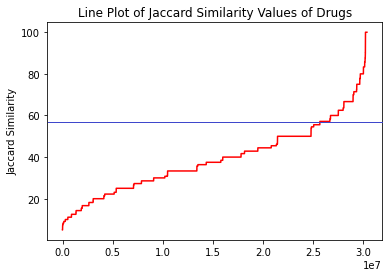
\includegraphics[width=0.5\linewidth]{chapters/materials_and_methods/figures/dds_line.png}
    \caption{Pairwise drug-drug Jaccard similarities.}
    \label{fig:dds}
\end{figure}

\subsection{Protein Related Information}
UniProt and STRING databases are the primary protein resources used in this thesis. We compile 505,250 proteins from the UniProt database, and more specifically, we compile 202,160 proteins belonging to the Homo sapiens and their amino acid sequences. We map 18,876 proteins to the STRING database and extract 183,746 protein-protein interaction information using the UniProt ID from the UniProt database. Finally, using the UniProt ID and Entrez Gene ID, we map the UniProt database to CTD and extract 32,495 protein-disease association information for 32,169 proteins and 126 distinct diseases.

Like the chemicals, in addition to protein-related information, we create a new relation named protein-protein similarity (PPS). Using the compiled amino acid sequences of proteins from the UniProt database, PPS data is obtained by calculating the similarity of these representations to each other according to the Jaccard Similarity of language units found by the BPE algorithm \cite{ozccelik2021debiaseddta}. Then, the similarity of the proteins was calculated in pairs according to the Jaccard Criterion using the formula given in Equation \ref{eq:jaccard}. By calculating the Jaccard Similarities of all protein-protein pairs, we obtained the values shown in Figure \ref{fig:pps}. Accordingly, protein pairs in the dataset with a similarity value greater than $9$ were determined to be similar to each other, with a threshold value was determined to cover at least $11\%$ of the whole data. In the end, we created 528 protein-protein similarity values for 465 distinct proteins.

\begin{figure}[h]
    \centering
        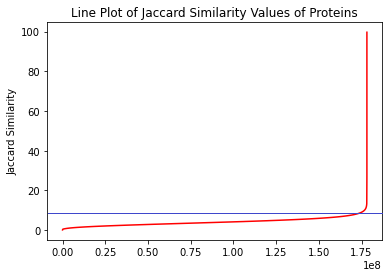
\includegraphics[width=0.5\linewidth]{chapters/materials_and_methods/figures/pps_line.png}
    \caption{Pairwise protein-protein Jaccard similarities.}
=======
>>>>>>> Stashed changes

% TO DO: Which information is used, jaccard vs also, lm
\section{Data Assembling}
\label{section:data_assembling}
Our idea was to represent chemicals and proteins better. Therefore, we compiled chemical and proteins related data from several online databases. And the challenging task was to assemble these compiled large data. For that purpose we analyze the available information in above mentioned databases and and map related information using common data. Figure \ref{fig:databases} shows used databases and the mapping IDs between corresponding databases.

\subsection{Chemical Related Information}
DrugBank, PubChem, and ChEMBL databases are the main resources of chemicals and we mainly focus on them. As an initial step we compile 14.350 drugs from DrugBank and retrieve their DrugBank IDs and InChI (International Chemical Identifier) Keys. Using InChI keys, we map the data in DrugBank to PubChem and ChEMBL databases and able to get the information about 10.935 distinct drugs. With 10.935 drugs, we extract 2.196.820 drug-drug relation information from DrugBank database. Using the PubChem CID (Compound ID number) information available at PubChem database, we map the PubChem to SIDER and CTD databases. From SIDER database, we extract 5452 distinct side effects and 115.871 drug-side effect association information for 1003 drugs. From CTD database, we extract 7086 distinct diseases and 995.654 drug-disease association information for 3387 drugs. Finally, using the InChI keys, we map DrugBank to ChEMBL and compile SMILES (Simplified molecular-input line-entry system) representations of 10.935 drugs. 

Apart from the already existing information we create a new relation, which we named as drug-drug similarity (DDS). Using the compiled SMILES representations of drugs from the ChEMBL (Davies et al., 2015) database, DDS data is obtained by calculating the similarity of these representations to each other according to the Jaccard Similarity Criterion. In order to find the similar SMILES sequences we used the Byte Pair Encoding (BPE) algorithm \cite{sennrich2015neural}. The BPE approach was utilized to identify the language unit vocabulary of chemicals. This method is commonly employed for discovering the tokens of a language, in the field of NLP. The BPE algorithm divided SMILES sequences into language units. Then, the similarity of the drugs was calculated in pairs according to the Jaccard Criterion using the formula given in Equation \ref{eq:jaccard}. By calculating the Jaccard Similarities of all drug-drug pairs, we obtained the values shown in Figure \ref{fig:dds}. Accordingly, drug pairs in the data set with a similarity value greater than $58$ were determined to be similar to each other with a threshold value was determined to cover at least $10\%$ of the whole data. In the end, we created 2.924.270 drug-drug similarity value for 6.963 distinct drugs.

\begin{equation}
    Jaccard (A, B) = \frac{A \cap  B}{ A \cup B} \times  100
\label{eq:jaccard}
\end{equation}

\begin{figure}
    \centering
        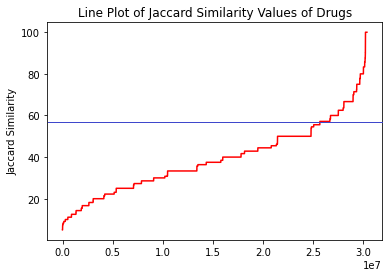
\includegraphics[width=0.5\linewidth]{chapters/materials_and_methods/figures/dds_line.png}
    \caption{Pairwise Drug-Drug Jaccard Similarities.}
    \label{fig:dds}
\end{figure}

%Given a corpus, all uni-characters are first considered as language units by the algorithm. The program then determines the total length of all pairs in the given text. The algorithm, now includes the most common two-character subsequences in the vocabulary. By treating each uni-characters in the vocabulary as a single character, this procedure continues until the goal vocabulary size is generated. The most frequently occurring subsequences of the necessary size are obtained when the method completes.

\subsection{Protein Related Information}
UniProt and STRING databases are main resources used in this thesis. We compile 505.250 proteins from the UniProt database and more specifically we compile 202.160 proteins belonging to the Homo sapiens, as well as their amino acid sequences. Using the UniProt ID from UniProt database, we map 18.876 proteins to STRING database, and extract 183.746 protein-protein interaction information. Finally, using the UniProt ID and Entrez Gene ID we map UniProt database to CTD and extract 32.495 protein-disease association information for 32.169 proteins and 126 distinct diseases.

Similar to the chemicals, besides the already existing protein-related information we create a new relation, which we named as protein-protein similarity (PPS). Using the compiled amino acid  sequences of proteins from the UniProt database, PPS data is obtained by calculating the similarity of these representations to each other according to the Jaccard Similarity Criterion. Again, we employ BPE algorithm to find the language units of protein sequences. Then, the similarity of the proteins was calculated in pairs according to the Jaccard Criterion using the formula given in Equation \ref{eq:jaccard}. By calculating the Jaccard Similarities of all protein-protein pairs, we obtained the values shown in Figure \ref{fig:pps}. Accordingly, protein pairs in the data set with a similarity value greater than $9$ were determined to be similar to each other with a threshold value was determined to cover at least $11\%$ of the whole data. In the end, we created 528 protein-protein similarity value for 465 distinct proteins.


\begin{figure}
    \centering
        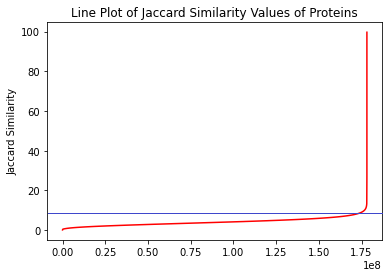
\includegraphics[width=0.5\linewidth]{chapters/materials_and_methods/figures/pps_line.png}
    \caption{Pairwise Protein-Protein Jaccard Similarities.}
<<<<<<< Updated upstream
=======
>>>>>>> d09ebba9e602d1522ef9361417dc21d129009597
>>>>>>> Stashed changes
    \label{fig:pps}
\end{figure}

\section{Graph Creation}
<<<<<<< HEAD
\label{section:graph_generation}
Graphs are used to model complex relations between entities and preserve structural information. In this study, we combine different types of data sources in order to predict binding affinity values between drug-target pairs by using the relevant drug and target-related information. For that purpose, we employ homogeneous and heterogeneous graphs which contain one type of node and relation or many types of nodes and relations, respectively. As discussed in the previous section, we compiled various data, extracted useful information, and then preprocessed them to use with the graph structure. Using PyTorch-Geometric \cite{fey2019fast}, we create graph structures that define node and edge types. Then, we load preprocessed data into graphs and generate positive and negative links between nodes. Observing the relations in the graphs, we sampled the metapaths as mentioned in Section \ref{section:graph_rep_le}. 

% \newpage
\newpage
\begin{table}
\centering
\caption{Homogeneous graph details.}
\vspace{0.25em}
\begin{tabular}{|l|c|c|c|} 
\hline
\multicolumn{1}{|c|}{\begin{tabular}[c]{@{}c@{}}Model\\Name\end{tabular}} & \begin{tabular}[c]{@{}c@{}}Number of\\Nodes\end{tabular} & Metapaths & \begin{tabular}[c]{@{}c@{}}Number of\\Edges\end{tabular} \\ 
\hline
Model (1), (2) & 10935 & Drug Interacts with Drug & 2196820 \\ 
\hline
Model (3), (4) & 6963 & Drug Similar to Drug & 5848540 \\ 
\hline
Model (5), (6) & 12675 & Protein Interacts with Protein & 124536 \\ 
\hline
Model (7), (8) & 465 & Protein Similar to Protein & 1056 \\
\hline
\end{tabular}
\label{tab:homo}
\end{table}

Table \ref{tab:homo} shows details about the Drug-Drug Interaction (DDI), Drug-Drug Similarity (DDS), Protein-Protein Interaction (PPI), and Protein-Protein Similarity (PPS) homogeneous graphs. For DDI relation, we created Model (1) and Model (2) graphs with 10,935 drug nodes and 2,196,820 edges between these nodes. While learning the representation of the graph, we follow the paths from drugs to drugs, so the name of the metapath is ``Drug interacts with the drug." In the case of DDS relation, we created Model (3) and Model (4) graphs with 6,963 drug nodes and 5,848,540 edges between these nodes. While learning the representation of the graph, similarly, we follow the paths from drugs to drugs, so the name of the metapath is ``Drug similar to the drug."


Similarly, we created Model (5) and Model (6) graphs for the PPI relation with 12,675 protein nodes and 124,536 edges between these nodes and the paths from proteins to proteins, with the metapath ``Protein interacts with the protein." Finally, we created Model (7) and Model (8) graphs for the PPS relation with 465 protein nodes and 1056 edges between these nodes, and the paths from proteins to proteins, with the metapath, ``Protein similar to the protein." 

% \newpage
\begin{table}
\centering
\caption{Heterogeneous graphs with disease information.}
\vspace{0.25em}
\begin{tabular}{|l|c|c|c|c|c|} 
\hline
\multicolumn{1}{|c|}{\begin{tabular}[c]{@{}c@{}}Model\\Name\end{tabular}} & \begin{tabular}[c]{@{}c@{}}Num.~of\\Drug\\Nodes\end{tabular} & \begin{tabular}[c]{@{}c@{}}Num. of\\Protein\\Nodes\end{tabular} & \begin{tabular}[c]{@{}c@{}}Num. of\\Disease\\Nodes\end{tabular} & Metapaths & \begin{tabular}[c]{@{}c@{}}Num. of\\Edges\end{tabular} \\ 
\hline
\begin{tabular}[c]{@{}l@{}}Model (9)\\Model (10)\end{tabular} & 3387 & - & 7086 & \begin{tabular}[c]{@{}c@{}}Drug Assoc. with Disease\\Disease Assoc. with Drug\end{tabular} & 1991308 \\ 
\hline
\begin{tabular}[c]{@{}l@{}}Model (11)\\Model (12)\end{tabular} & - & 32169 & 126 & \begin{tabular}[c]{@{}c@{}}Protein Assoc.with Disease\\Disease Assoc.with Protein\end{tabular} & 64990 \\ 
\hline
\begin{tabular}[c]{@{}l@{}}Model (13)\\Model (14)\end{tabular} & 3387 & 32169 & 7087 & \begin{tabular}[c]{@{}c@{}}Drug Assoc. with Disease\\Disease Assoc.with Protein\\Protein Assoc.with Disease\\Disease Assoc.with Drug\end{tabular} & 2056298 \\
\hline
\end{tabular}
\label{tab:het_disease}
\end{table}
Creating heterogeneous graphs needs more effort since the relations between them can be complicated, and the number of information drastically increases the run time. After creating homogeneous graphs, we create heterogeneous graphs using available disease association information. 

\newpage
Table \ref{tab:het_disease} shows details about the Drug-Disease Association (DDiA), Protein-Disease Association (PDiA), and Drug-Disease-Protein Association (DDiPA) heterogeneous graphs. For DDiA relation, we created Model (9) and Model (10) graphs with 3,387 drug nodes, 7,086 disease nodes, and 21,991,308 edges between these nodes. While learning the representation of the graph, we follow the paths from drugs to diseases and vice versa, so the metapaths are ``Drug associates with a disease," and ``Disease reversely associates with a drug." The distinction between the two models is the integration of language models into Model (10) in order to enrich the representation of drugs. Like the DDiA, for the PDiA relation, we created Model (11) and Model (12) graphs with 32,169 protein nodes, 126 disease nodes, and 64,990 edges between these nodes. We follow the paths from proteins to diseases and the reverse paths, so the metapaths are ``Protein associates with a disease," and ``Disease reversely associates with a protein." Similar to Model (10), Model (12) also employs language models. Finally, we combine these two heterogeneous graphs and create one extensive heterogeneous network. Model (13) and Model (14) graphs for the DDiPA relation with 3,387 drug nodes, 6,963 protein nodes, 7087 disease nodes, and 2,056,298 edges between these three nodes. We follow the paths as drug-disease-protein-disease-drug, with the metapaths ``Drug associates with a disease," ``Disease reversely associates with a protein," ``Protein associates with a disease," and ``Disease reversely associates with a drug." To sum up, Model (13) combines the relations between drugs-diseases and proteins-diseases, and Model (14) uses the same types of nodes and relations; however, it integrates language model approaches for biomolecules and diseases to enrich the drug-target representations. 

As an additional experiment, we create another set of models and test the effectiveness of side effect information with these models. Table \ref{tab:het_se} gives details about the Drug-Side Effect Association (DSA) and DDI with DSA heterogeneous graphs. For the DSA graph, we created Model (15) and Model (16) graphs with 1.003 drug nodes, 5,451 side effect nodes, and 231,742 edges between these nodes. While learning the representation of the graph, we follow the paths from drugs to side effects and vice versa, so the metapaths are ``Drug associates with a side effect" and ``Side effect reversely associates with a drug."  DDI is created as in the case of Model (1) and Model (2). For the combination of DDI and DSA graphs, we created Model (17) and Model (18) graphs with 10,932 drug nodes, 5,451 side effect nodes, and 2,427,902 edges between these nodes. We follow the paths from drugs to side effects, side effects to drugs, and drugs to drugs, so the metapaths are ``Drug associates with a side effect," ``Side effect reversely associates with a drug," and ``Drug interacts with a drug." Both Model (16) and Model (18) integrate language models for drugs and side effects.

% \newpage
In order to incorporate language models into the graphs, we used three language model-based representation learning algorithms, namely ProtBERT, ChemBERTa, and BioBERT. 
ProtBERT is a transformer-based model with a masked language modeling objective with 30 layers and 16 attention heads. For each protein sequence, it generates a 1024-length vector as
\begin{equation}
    PB^{t} = \left[\begin{array}{cccccc} pb_1^{t} & pb_2^{t} & pb_3^{t} & \ldots & pb_1014^{t} \end{array} \right].
\end{equation}

\newpage
ProtBERT is based on the BERT model, which is self-supervised and has been pre-trained on a large number of protein sequences. The ProtBERT model is used to initialize the distributional representations of proteins.
=======
% TO DO: Insert node edge numbers, types
% pos and neg edge sampling
\subsection{Homogeneous Graphs}



\subsection{Heterogeneous Graphs}


\section{Learning Distributional Vector Representations}
Machine learning on graph structured data is a ubiquitous task and one of the challenges of this task is to find a way to represent the structure itself and the information it holds so that it can be easily interpreted by mostly used machine learning models. In this thesis, we employ metaPath2Vec \cite{dong2017metapath2vec} model and learn the graph-based distributional representation vectors that reflect the semantic connections in the graph for nodes and edges and finally represent data that cannot be expressed in Euclidean space as a graph.
<<<<<<< Updated upstream
=======
>>>>>>> d09ebba9e602d1522ef9361417dc21d129009597
>>>>>>> Stashed changes

\begin{table}
\centering
\caption{Heterogeneous graphs with side effect information.}
\vspace{0.25em}
\begin{tabular}{|l|c|c|l|c|} 
\hline
\multicolumn{1}{|c|}{\begin{tabular}[c]{@{}c@{}}Model\\Name\end{tabular}} & \begin{tabular}[c]{@{}c@{}}Number\\of~Drug\\Nodes\end{tabular} & \begin{tabular}[c]{@{}c@{}}Number of\\Side~Effect\\Nodes\end{tabular} & \multicolumn{1}{c|}{Metapaths} & \begin{tabular}[c]{@{}c@{}}Number\\of Edges\end{tabular} \\ 
\hline
\begin{tabular}[c]{@{}l@{}}Model (15),\\Model (16)\end{tabular} & 1003 & 5451 & \begin{tabular}[c]{@{}l@{}}Drug Associates with Side Effect\\Side Effect Associates with Drug\end{tabular} & 231742 \\ 
\hline
\begin{tabular}[c]{@{}l@{}}Model (17)\\Model (18)\end{tabular} & 10935 & 5451 & \begin{tabular}[c]{@{}l@{}}Drug Associates with Side Effect\\Side Effect Associates with Drug\\Drug Interacts with Drug\end{tabular} & 2427902 \\
\hline
\end{tabular}
\label{tab:het_se}
\end{table}

To initialize the distributed representations of chemicals, we used the ChemBERTa model pre-trained on 10M PubChem substances using BPE tokenization. ChemBERTa is built on the transformer, has 12 attention heads and six layers, and is pre-trained with masked language modeling.

The BioBERT model was used to initialize the distributed representations of diseases and side effects. Like the previous models, it is a domain-specific language representation model that's been pre-trained on large-scale biological corpora.

<<<<<<< Updated upstream
=======
<<<<<<< HEAD
\section{Learning Distributed Vector Representations}
Representation learning has provided a novel learning paradigm for AI domains. The subject of representation learning is examined and demonstrated in this study, focusing on homogeneous and heterogeneous networks, which contain one type of node and relations or many types of nodes and relations, respectively. The objective of this problem is to automatically project nodes in networks into latent embedding space so that the network's structural and relational properties can be encoded and preserved. Machine learning algorithms can then employ embeddings as features to address relevant downstream machine learning tasks. 
=======
>>>>>>> Stashed changes
% cosine similarity ile val evaluation
% hepsinin sonuclari
>>>>>>> d09ebba9e602d1522ef9361417dc21d129009597

%The majority of heterogeneous network representation learning approaches are inspired by and developed based on homogeneous network representation learning. The primary question is how to encode both the structural and semantic aspects of networks by transforming the structures between different types of nodes and edges into latent spaces. 

Machine learning on graph-structured data is a ubiquitous task, and one of the challenges of this task is to find a way to represent the structure itself and the information it holds so that mainly used machine learning models can easily interpret it. In this thesis, we employ Metapath2Vec \cite{dong2017metapath2vec} model and learn the graph-based distributed representation vectors that reflect the semantic connections in the graph for nodes and edges and finally represent data that cannot be expressed in Euclidean space as a graph.

Metapath2Vec uses priori paths as its basic operating principle, so the paths should be defined in advance, as described in Section \ref{section:graph_rep_le}. Metapath2Vec evaluates different types of edge relations while finding meta paths, that is, paths going from one node to another node, provided that they do not repeat it, and makes semantic inferences using these edges and uses them in vector representations.

ProtBERT and ChemBERTa pre-trained language models are also employed to enrich the distributed vector representations of drugs and proteins learned from the Metapath2Vec algorithm. To do that, we initialize each biomolecule's embeddings with the corresponding vector from pre-trained language models, then start Metapath2Vec's training.

\section{WideDeepDTA}
WideDeepDTA aims to predict binding affinity values of drug-target pairs using information-rich representation vectors of corresponding drugs and targets. In order to generate rich representations, it combines text-based features with network and language model-based representation learning approaches. WideDeepDTA comprises three components, (i) CNN-based DeepDTA model, (ii) graph representation learning, and (iii) affinity prediction.


\subsection{DeepDTA Model}
DeepDTA is an affinity prediction model that uses chemicals' SMILES strings and proteins' amino-acid sequences to represent biomolecules. To represent each character of SMILES and protein sequences, it leverages integer/label encoding with 64 and 25 unique letters, respectively. For instance, the SMILES string ``$ [ C \;\; N \;\;=\;\; C\;\; =\;\; O]$'' is encoded as $[ 1 \;\; 3 \;\; 63\;\; 1 \;\;63\;\; 5]$. Once label encodings are generated, Keras' Embedding Layer is applied to represent characters as 128-dimensional dense vectors. Embeddings are fed into CNN blocks with three 1D-convolutional layers, followed by max-pooling layers. The final feature vectors of SMILES strings and proteins sequences are concatenated and fed into three fully connected neural networks.

\section{Graph Representation Learning}
WideDeepDTA modifies the DeepDTA model and makes it wider. To do that, it combines four input types, namely  SMILES representation and protein sequence representation generated by CNN Blocks; chemical embeddings and protein embeddings generated by graph representation learning. Figure \ref{fig:widerdeepdta} illustrates the overall process. In this section, we explain the details of the WideDeepDTA model.
\begin{figure}
    \centering
        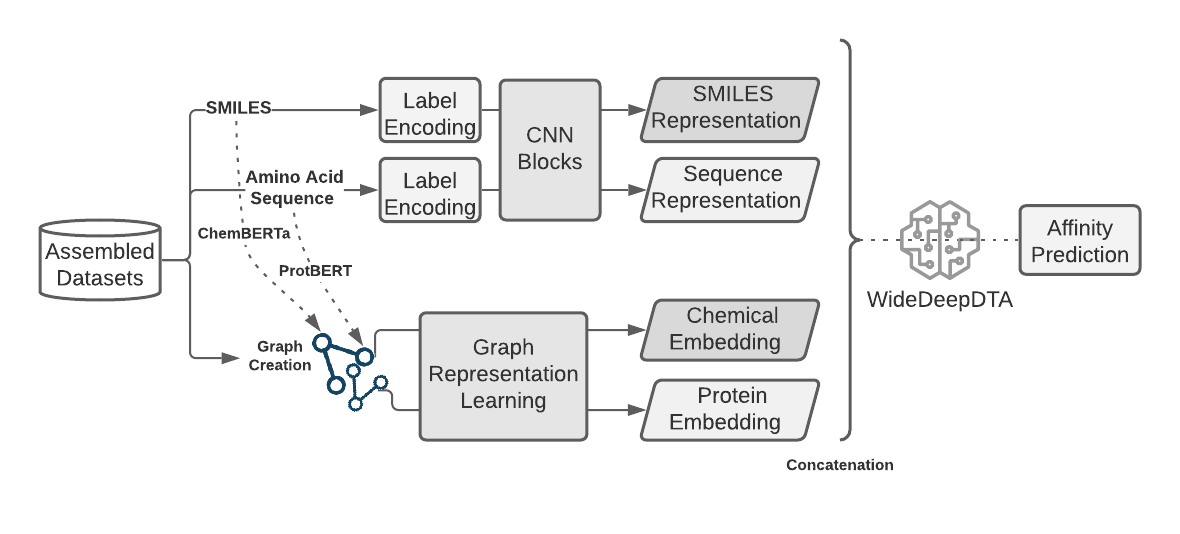
\includegraphics[width=\linewidth]{chapters/materials_and_methods/figures/WiderDeep.png}
    \caption{WideDeepDTA summarized.}
    \label{fig:widerdeepdta}
\end{figure}

After compiling and assembling the datasets, we create our graphs. We define several homogeneous and heterogeneous graphs augmented with the drug and target-related relations explained in Chapter \ref{results}. An example heterogeneous graph is a Drug-Disease-Protein Association (DDiPA) graph. The DDiPA graph $DDiPA(V,\varepsilon))$ consists of a set of drugs $D = {D_1, D_2, …, D_n}$ of $n$ drug nodes, set of targets $T = {P_1, P_2, …, P_m}$ of m protein nodes, and $Di = {Di_1, Di_2, …, Di_t}$ of $t$ disease nodes. DDiPA graph contains two types of edges. The first type of edge represents the association between drug and disease nodes, and the edge from this type is named ``Drug Associates with a Disease." The second type of edge represents the association between protein and disease nodes, and the edge from this type is named ``Protein Associates with a Disease." 

Once the DDiPA graph is created, we load the edges (\textit{i.e.,} positive edges) using drug-disease and protein disease association data extracted from the SIDER database. We split the graph into training and validation sets, in which the validation set contains at least 5\% of the data. Then, we construct the negative samples by generating all possible pairs between drug-disease and protein-disease pairs, then selecting a sample from pairs as many as the number of positive edges in a validation set. Generating negative samples means introducing unknown interactions to the graph to prevent overfitting.

\section{Experimental Setup}
For the whole study, we used Python programming language and performed experiments on Google Colaboratory \cite{carneiro2018performance}, and a machine with NVIDIA Tesla V100 GPU and Intel Xeon Scalable 6148 CPU.

As the training and test folds, we use the same setup in the DeepDTA model. We train each model 5 times with the training set folds, measure the performance on each test set, and report the average results on the BDB dataset. The BDB dataset contains five different training sets and corresponding four different test sets: warm, cold ligand, cold protein, and cold both. The cold ligand test set is used to identify the interactions between unknown ligands and known proteins, \textit{i.e.,} biomolecules that are not used during the training, biomolecules that are used during the training, respectively. The cold protein test set identifies the interactions between known ligands and unknown proteins. Identifying the interactions between known biomolecules form the warm test set, and finally, the interactions between unknown biomolecules form the cold both test set. However, some information related to biomolecules listed as unknown in the test set can be present in the graph creation part. We compute each model's CI, MSE, RMSE, and $R^2$ scores and report the standard deviation in parentheses.

\section{Hyper-parameter Search}
In order to learn distributed representation vectors of chemicals and proteins using the created graphs, we employed the Metapath2Vec model. The Metapath2Vec model uses the train set to train several hyper-parameters such as the embedding size of each embedding vector, walk length throughout the metapath, context size, which is considered for positive samples, and the number of walks to sample for each node in order to find the best model that generated the most convenient representations for the corresponding dataset. The model uses two initialization approaches; (i) random initialization and (ii) initialization using pre-trained language models. In the former case, each node is represented with 32-dimensional vectors initialized as samples from a uniform distribution over $[0,1)$, and in the latter case, each node is represented with 32-dimensional vectors initialized by the pre-trained language models. For that purpose, we used ChemBERTa and ProtBERT pre-trained language models and loaded the embeddings of chemicals and proteins used in the creation of graphs. We also leveraged BioBERT, which is used by the disease names and side effect names associated with the drugs and proteins. In both cases, training goes for 100 epochs, and the model tests the best set of parameters over the validation set. We calculate the training and the validation loss to see the model's performance. 

Since we aim to create better representation for drugs and proteins, we test the success of representations using the cosine similarity metric. Therefore, we first calculate the cosine similarity of positive edges and the cosine similarity of negative edges. Then observe the difference between these two calculations to see whether the model is good at learning the representations or not. In the end, the model sticks with the graph that gives the highest total cosine similarity value. 

Finally, we obtained the low-dimensional representation vectors for each chemical and protein node in the graph. Later on, we concatenate low-dimensional representation vectors of chemicals and proteins generated by the Metapath2Vec algorithm with the representation vectors generated by the CNN blocks. Like the DeepDTA model, combined representation is fed into three fully connected layers. We used 1024 nodes in the first two fully connected layers, followed by a dropout layer of rate $0.1$. The last fully-connected layer contains 512 nodes, followed by the output layer. The proposed model that combines CNN and network-based methods is illustrated in Figure \ref{fig:widedeepdtamodel}.

% \newpage
\section{Affinity Prediction}
Similar to the DeepDTA, the WideDeepDTA model handles the drug-target binding affinity prediction task as a regression problem, using Rectified Linear Unit (ReLU) \cite{nair2010rectified} as the activation function and MSE as the loss function. With MSE, the model aims to maximize the difference between the actual and the predicted value during training. In the case of the CNN-based model, the Adam optimization algorithm \cite{kingma2014adam} is used. In the case of the network-based model
% , the lazy version of the Adam algorithm, namely
SparseAdam is employed. 

\begin{figure}[t]
    \centering
        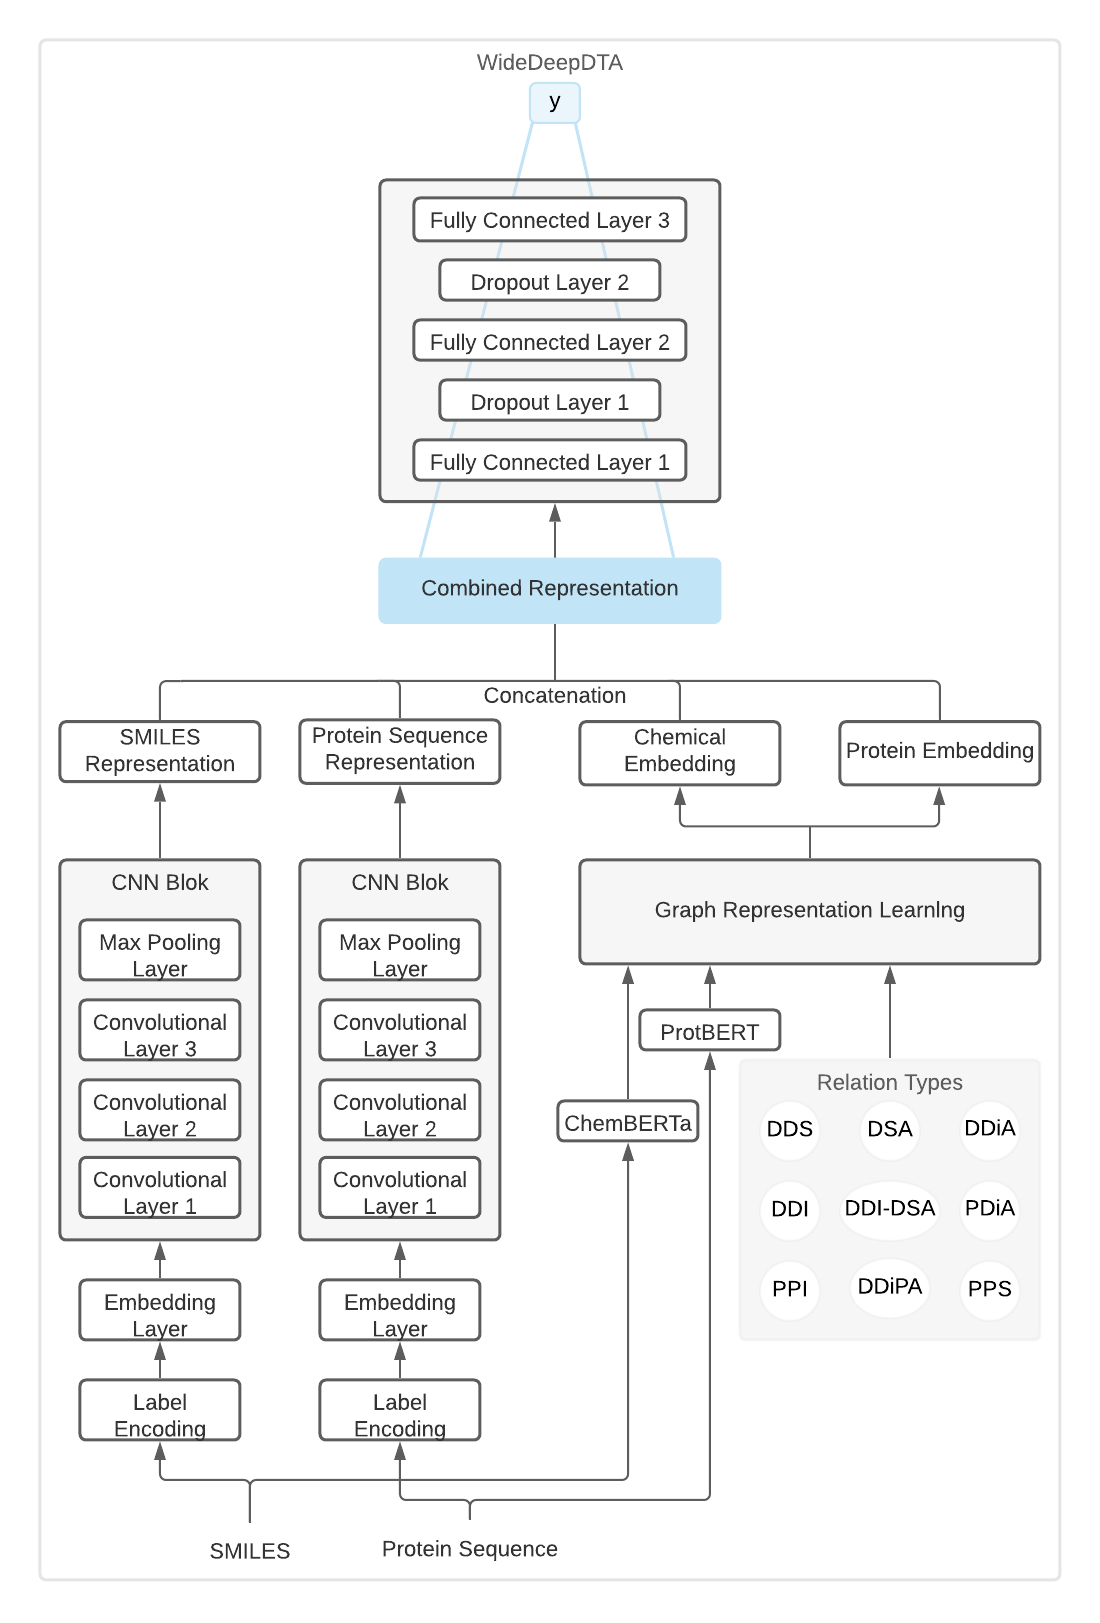
\includegraphics[width=\linewidth]{chapters/materials_and_methods/figures/WiderDeepDTA Model.png}
    \caption{WideDeepDTA in details.}
    \label{fig:widedeepdtamodel}
\end{figure}


<<<<<<< HEAD
% Overall yorumum su: baya guzel bir materyal var burda. Yazdikca yazim kaliten acilmis bence :D Yalniz bu materyal hala biraz daginik. Bence basliklarin yeri degismeli ve sayisi artmali. Basliklarin altindaki bazi materyaller de tam tutmuyor. Re-organize edersen baya duzelecek bence. 
=======
\section{WiderDeepDTA}
In WideDeepDTA, we empowered heterogeneous networks using language models. 
% explain used machines.


\begin{figure}
    \centering
        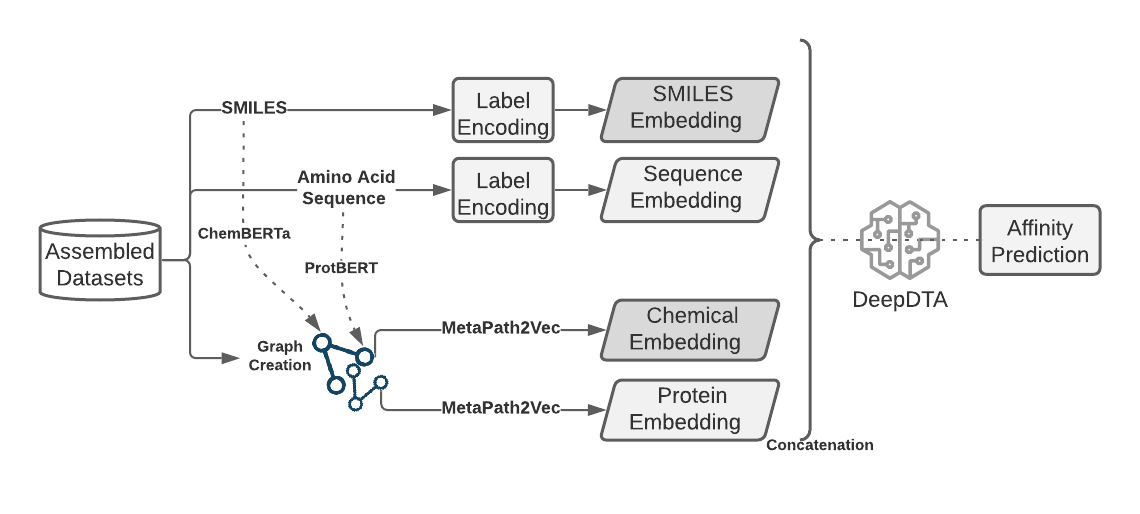
\includegraphics[width=\linewidth]{chapters/materials_and_methods/figures/WiderDeepDTA.png}
    \caption{WideDeepDTA Summarized.}
    \label{fig:widerdeepdta}
\end{figure}


\begin{figure}
    \centering
        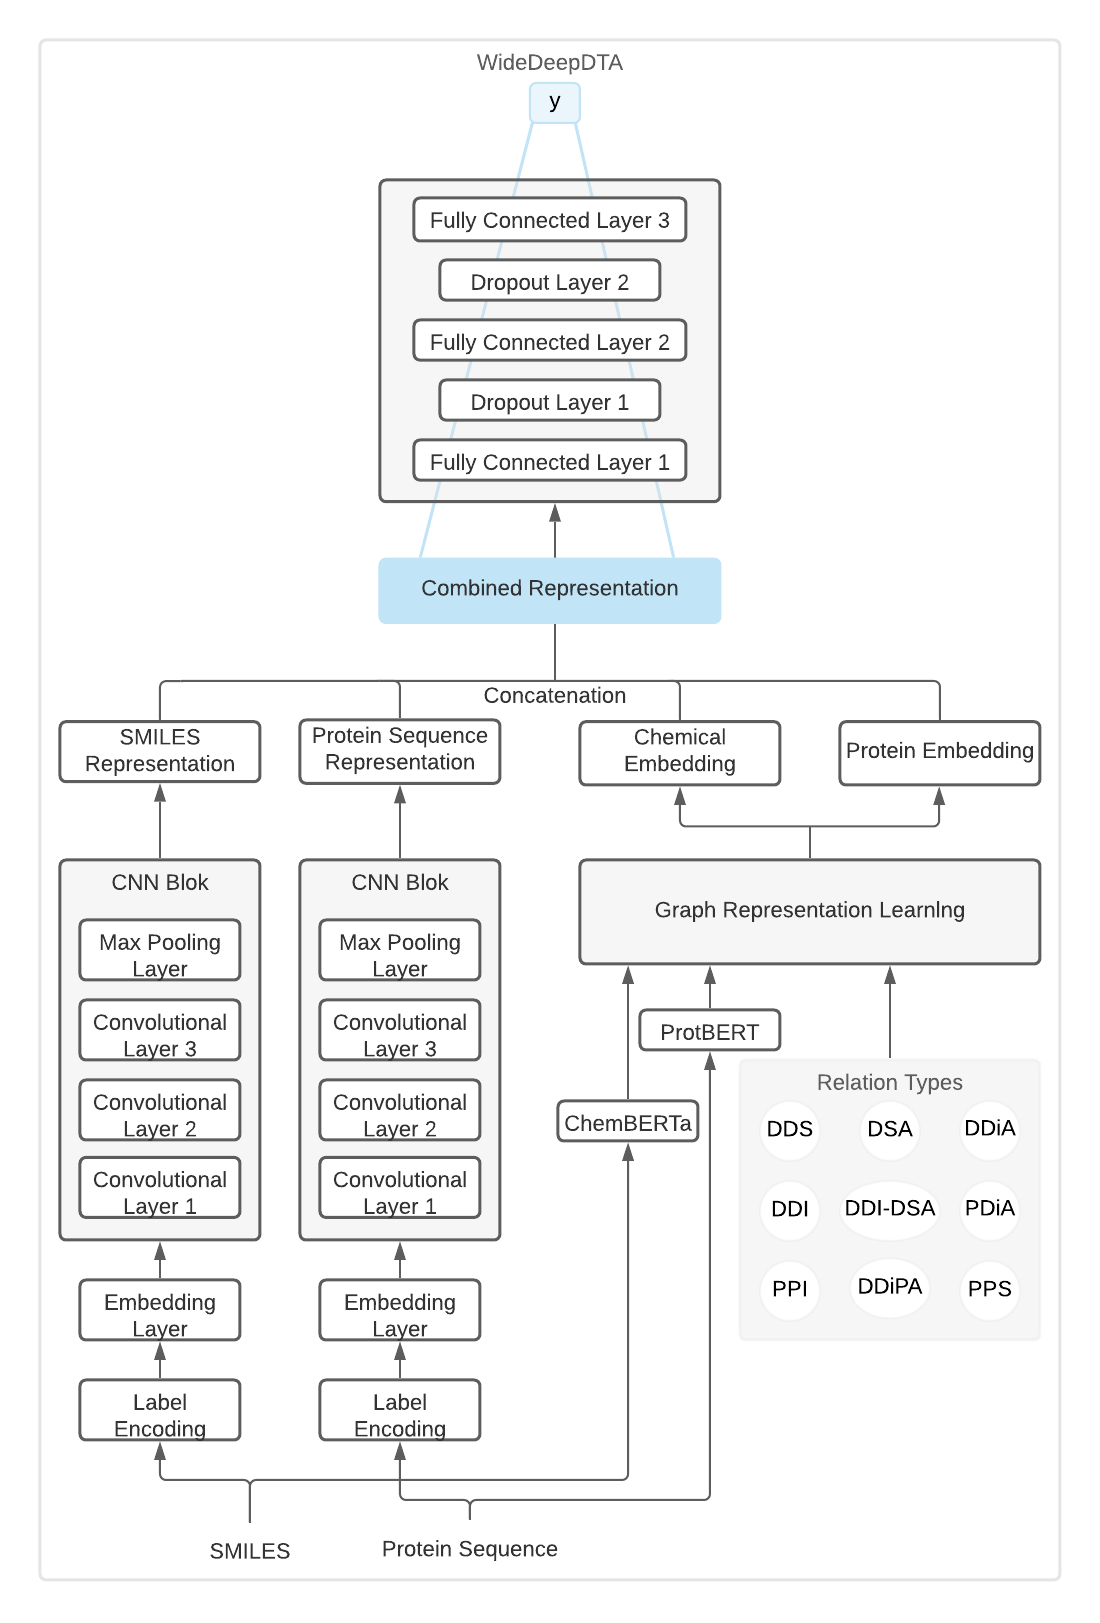
\includegraphics[width=\linewidth]{chapters/materials_and_methods/figures/WiderDeepDTA Model.png}
    \caption{WideDeepDTA in Details.}
    \label{fig:widedeepdtamodel}
<<<<<<< Updated upstream
\end{figure}
=======
\end{figure}
>>>>>>> d09ebba9e602d1522ef9361417dc21d129009597
>>>>>>> Stashed changes

\chapter{RESULTS}

\section{Evaluation}
Representation vectors for chemicals and proteins obtained using the aforementioned models and graphs, and then these vectors evaluated in the drug-target affinity task with the DeepDTA model using the BDB dataset. The DeepDTA model represents proteins using amino acid sequences and chemicals using characters of the SMILES notations. In this study, the DeepDTA model has been updated, as shown in Figure 3.3, to take as input the representation vectors containing additional information in the generated graphs. The performance of the model is measured by the Concordance Index (CI),  Mean Squared Error (MSE), Root Mean Squared Error (RMSE), and $R2$ metrics. 

% explain metrics with formula

\section{Experimental Setup}

As the training and test folds we use the same setup used in DeepDTA \cite{ozturk2018deepdta}. We train each model 5 times with the training set folds, then measure the performance on each test set, and report the average results on BDB. BDB dataset contains 5 different training sets and corresponding 4 different test sets as warm, cold ligand, cold protein and cold. The cold test sets contain data that was not used during the training of the model. We compute CI, MSE, RMSE, and $R^2$ scores of each model and report with the standard deviation.


\section{Model Comparisons}

\paragraph{Homogeneous ligand representation}
First, we generate homogeneous graphs with only one node and edge type, then test WideDeepDTA performance for the ligand representation.

\begin{itemize}
    \item \textbf{Model (1)}: A DDI (Drug-Drug Interaction) graph is created, the nodes of which are formed by all drugs (D) and the edges by interactions (D-D) between these drugs.   
    \item \textbf{Model (2)}: A DDI graph is created similar to Model (1), this time with the knowledge of initial embeddings of ChemBERTa model.
    \item \textbf{Model (3)}: A DDS (Drug-Drug Similarity) graph is created, the nodes of which are formed by all drugs (D) and the edges by Jaccard similarity between these drugs. 
    \item \textbf{Model (4)}: A DDS graph is created similar to Model (3), this time with the knowledge of initial embeddings of ChemBERTa model.
\end{itemize}

We first test the impact of ligand representation using homogeneous graphs by creating two different models with two different versions. Model (1) represents each drug with a 32-dimensional vector in which they are initialized as samples
from a uniform distribution over $[0, 1)$ and trained by metapath2vec model on DDI relation, and Model (2) represents each drug with the same dimensional size vector, however metapath2vec model's embeddings are initialized as ChemBERTa embeddings of corresponding ligands. (For the detailed results please refer to the Appendix \ref{app:homogeneous_ligand} and see Table \ref{tab:ddi_ci_r2} and Table \ref{tab:ddi_mse_rmse}.) On the other hand, Model (3) and Model (4) are trained on DDS relation with the same setup. (For the detailed results please refer to the Appendix \ref{app:homogeneous_ligand} and see Table \ref{tab:dds_ci_r2} and Table \ref{tab:dds_mse_rmse}.)

The results regarding the comparison of these four models are shown in Table \ref{tab:ddi_vs_dds_warm}, Table \ref{tab:ddi_vs_dds_cold_prot}, Table \ref{tab:ddi_vs_dds_cold_ligand}, and Table \ref{tab:ddi_vs_dds_cold_both}. Considering the results shown in Table \ref{tab:ddi_vs_dds_warm};
\begin{itemize}
    \item DDI models and DDS models perform similarly on the warm test set of BDB, \textit{i.e.}, their trends are the same for the same performance metrics. For instance, value of $R^2$ for models with PLMs is higher than the randomly initialized models, likewise MSE and RMSE values are lower for DDI and DDS models for the same case.
    \item Using PLM for drugs actually works since it increases the performance for three out of four metrics for both of the DDI and DDS models.
    \item As a result, we claim that, one can employ the similarity measures between two drugs when the interaction information is not available for these two drugs while using empowered homogeneous graphs on warm test set of BDB.
\end{itemize}

\begin{table}[H]
\centering
\caption{Scores of DDI and DDS models on \textbf{warm} test set of BDB.}
\label{tab:ddi_ci_r2}
\begin{tabular}{|l|l|c|l|l|} 
\hline
Model & \multicolumn{1}{c|}{CI} & $R^2$ & \multicolumn{1}{c|}{MSE} & \multicolumn{1}{c|}{RMSE} \\ 
\hline
DeepDTA & 0.888 (0.009) & 0.781 (0.028) & 0.288 (0.021) & 0.536 (0.012) \\ 
\hline
Model (1) & \textbf{0.896 (0.009)} & 0.777 (0.026) & 0.295 (0.036) & 0.542 (0.033) \\ 
\hline
Model (2) & 0.890 (0.014) & 0.782 (0.017) & 0.287 (0.014) & 0.535 (0.014) \\ 
\hline
Model (3) & 0.893 (0.005) & 0.787 (0.020) & 0.280 (0.017) & 0.529 (0.017) \\ 
\hline
Model (4) & 0.890 (0.006) & \textbf{0.789 (0.008)} & \textbf{0.278 (0.011)} & \textbf{0.527 (0.010)} \\
\hline
\end{tabular}
\label{tab:ddi_vs_dds_warm}
\end{table}


As stated in the work of DeepDTA, CNN's ability to represent protein sequences is very low \cite{ozturk2018deepdta}. We initialized all the protein embeddings with zeros, since we do not train our models with any kinds of protein-related information. Considering the results shown in Table \ref{tab:ddi_vs_dds_cold_prot}, even initializing with zeros increases the performance for the DDI model. 


\begin{table}[H]
\centering
\caption{Scores of DDI and DDS models on \textbf{cold protein} test set of BDB.}
\label{tab:ddi_ci_r2}
\begin{tabular}{|l|l|c|l|l|} 
\hline
Model & \multicolumn{1}{c|}{CI} & $R^2$ & \multicolumn{1}{c|}{MSE} & \multicolumn{1}{c|}{RMSE} \\ 
\hline
DeepDTA & 0.759 (0.006) & 0.315 (0.049) & 1.085 (0.146) & 1.040 (0.146) \\ 
\hline
Model (1) & \textbf{0.779 (0.030)} & \textbf{0.375 (0.104)} & \textbf{0.992 (0.207)} & \textbf{0.991 (0.101)} \\ 
\hline
Model (2) & 0.768 (0.009) & 0.327 (0.072) & 1.064 (0.154) & 1.029 (0.077) \\ 
\hline
Model (3) & 0.775 (0.018) & 0.340 (0.082) & 1.045 (0.174) & 1.019 (0.086) \\ 
\hline
Model (4) & 0.774 (0.015) & 0.327 (0.075) & 1.065 (0.162) & 1.029 (0.079) \\
\hline
\end{tabular}
\label{tab:ddi_vs_dds_cold_prot}
\end{table}

Taking into consideration the results shown in Table \ref{tab:ddi_vs_dds_cold_ligand} and Table \ref{tab:ddi_vs_dds_cold_both}, adding drug-related information using the homogeneous graph or empowered homogeneous graph did not improve the performance for the cold ligand and cold both test cases. However, results for cold both test set slightly better then the cold ligand test set due to the performance improvement of cold proteins. 

<<<<<<< Updated upstream
=======
<<<<<<< HEAD
\begin{table}
\centering
\caption{Scores of DDI and DDS models on cold ligand test set of BDB.}
\vspace{0.25em}
=======
>>>>>>> Stashed changes
\begin{table}[H]
\centering
\caption{Scores of DDI and DDS models on \textbf{cold ligand} test set of BDB.}
\label{tab:ddi_ci_r2}
<<<<<<< Updated upstream
=======
>>>>>>> d09ebba9e602d1522ef9361417dc21d129009597
>>>>>>> Stashed changes
\begin{tabular}{|l|l|c|l|l|} 
\hline
Model & \multicolumn{1}{c|}{CI} & $R^2$ & \multicolumn{1}{c|}{MSE} & \multicolumn{1}{c|}{RMSE} \\ 
\hline
DeepDTA & \textbf{0.687 (0.096)} & \textbf{0.039 (0.243)} & \textbf{1.448 (0.939)} & \textbf{1.152 (0.348)} \\ 
\hline
Model (1) & 0.664 (0.057) & -0.053 (0.210) & 1.472 (0.650) & 1.187 (0.249) \\ 
\hline
Model (2) & 0.640 (0.066) & -0.125 (0.180) & 1.548 (0.602) & 1.225 (0.220) \\ 
\hline
Model (3) & 0.651 (0.085) & -0.139 (0.132) & 1.603 (0.645) & 1.242 (0.246) \\ 
\hline
Model (4) & 0.666 (0.064) & -0.102 (0.330) & 1.502 (0.615) & 1.202 (0.239) \\
\hline
\end{tabular}
\label{tab:ddi_vs_dds_cold_ligand}
\end{table}
<<<<<<< Updated upstream
=======
<<<<<<< HEAD
\begin{table}
\centering
\caption{Scores of DDI and DDS models on cold both test set of BDB.}
\vspace{0.25em}
=======
>>>>>>> Stashed changes
\begin{table}[H]
\centering
\caption{Scores of DDI and DDS models on \textbf{cold both} test set of BDB.}
\label{tab:ddi_ci_r2}
<<<<<<< Updated upstream
=======
>>>>>>> d09ebba9e602d1522ef9361417dc21d129009597
>>>>>>> Stashed changes
\begin{tabular}{|l|l|c|l|l|} 
\hline
Model & \multicolumn{1}{c|}{CI} & $R^2$ & \multicolumn{1}{c|}{MSE} & \multicolumn{1}{c|}{RMSE} \\ 
\hline
DeepDTA & \textbf{0.554 (0.047)} & \textbf{-0.154 (0.164)} & \textbf{2.007 (1.223)} & \textbf{1.356 (0.410)} \\ 
\hline
Model (1) & 0.554 (0.044) & -0.287 (0.184) & 2.013 (0.767) & 1.395 (0.260) \\ 
\hline
Model (2) & 0.495 (0.037) & -0.496 (0.211) & 2.348 (0.978) & 1.504 (0.294) \\ 
\hline
Model (3) & 0.519 (0.036) & -0.390 (0.235) & 2.278 (1.069) & 1.467 (0.356) \\ 
\hline
Model (4) & 0.536 (0.068) & -0.274 (0.269) & 2.021 (0.950) & 1.388 (0.308) \\
\hline
\end{tabular}
\label{tab:ddi_vs_dds_cold_both}
\end{table}

\paragraph{Homogeneous protein representation}
Second, we generate homogeneous graphs with only one node and edge type, then test WideDeepDTA performance for the protein representation.

\begin{itemize}
    \item \textbf{Model (5)}: A PPI (Protein-Protein Interaction) graph is created, the nodes of which are formed by all proteins (P) and the edges by interactions (P-P) between these proteins.   
    \item \textbf{Model (6)}: A PPI graph is created similar to Model (3), this time with the knowledge of initial embeddings of ProtBERT model.
    \item \textbf{Model (7)}: A PPS (Protein-Protein Similarity) graph is created, the nodes of which are formed by all proteins belonging to the human species (P) and the edges formed by the Jaccard similarities (P-P) between the amino acid sequences of these proteins. While calculating the similarities we tokenized each amino acid sequence using the glossary generated by BPE. Then we calculate the Paired Jaccard similarities of protein tokens. Considering the dataset, a threshold value is determined to cover at least 11\% of the data. Accordingly, protein pairs with similarity values greater than 9 determined to be similar to each other. 
    \item \textbf{Model (8)}: A PPS graph is created similar to Model (7), this time with the knowledge of initial embeddings of ProtBERT model.
\end{itemize}

First, we test the impact of protein representation using homogeneous graphs by creating two different models with two different versions. Model (5) represents each protein with a 32-dimensional vector in which they are initialized as samples from a uniform distribution over $[0, 1)$ and trained by metapath2vec model on PPI relation, and Model (6) represents each drug with the same dimensional size vector, however metapath2vec model's embeddings are initialized as ProtBERT embeddings of corresponding proteins. (For the detailed results please refer to the Appendix \ref{app:homogeneous_protein} and see Table \ref{tab:ppi_ci_r2} and Table \ref{tab:ppi_mse_rmse}.) On the other hand, Model (7) and Model (8) are trained on PPS relation with the same setup. (For the detailed results please refer to the Appendix \ref{app:homogeneous_protein} and see Table \ref{tab:pps_ci_r2} and Table \ref{tab:ppse_mse_rmse}.)

The results regarding the comparison of these four models are shown in Table \ref{tab:ppi_vs_pps_warm}, Table \ref{tab:ppi_vs_pps_cold_protein}, Table  \ref{tab:ppi_vs_pps_cold_ligand}, and Table \ref{tab:ppi_vs_pps_cold_both}. Considering the results shown in Table \ref{tab:ppi_vs_pps_warm};
\begin{itemize}
    \item Empowered graphs generated by PPS relation adds more information to the representation of proteins compared to the empowered graphs generated by PPI relation on warm test set. 
    \item In the case of PPI models, model with empowered graph performs better than the normal graphs in all metrics, except CI. However, both of them perform worse than the DeepDTA model on warm test set.
\end{itemize}

Considering the results shown in Table \ref{tab:ppi_vs_pps_cold_protein};
\begin{itemize}
    \item Empowered graphs generated by PPS relation adds more information to the representation of proteins compared to the empowered graphs generated by PPI relation on warm test set. 
    \item In the case of PPI models, model with empowered graph performs better than the normal graphs in all metrics, except CI. However, both of them perform worse than the DeepDTA model on warm test set.
\end{itemize}

<<<<<<< Updated upstream
=======
<<<<<<< HEAD
\begin{table}
\centering
\caption{Scores of PPI and PPS models on warm test set of BDB.}
\vspace{0.25em}
=======
>>>>>>> Stashed changes
\begin{table}[H]
\centering
\caption{Scores of PPI and PPS models on \textbf{warm} test set of BDB.}
\label{tab:ddi_ci_r2}
<<<<<<< Updated upstream
=======
>>>>>>> d09ebba9e602d1522ef9361417dc21d129009597
>>>>>>> Stashed changes
\begin{tabular}{|l|l|c|l|l|} 
\hline
Model & \multicolumn{1}{c|}{CI} & $R^2$ & \multicolumn{1}{c|}{MSE} & \multicolumn{1}{c|}{RMSE} \\ 
\hline
DeepDTA & 0.888 (0.009) & 0.781 (0.028) & 0.288 (0.021) & 0.536 (0.012) \\ 
\hline
Model (5) & 0.888 (0.009) & 0.773 (0.025) & 0.299 (0.020) & 0.546 (0.018) \\ 
\hline
Model (6) & 0.888 (0.009) & 0.777 (0.012) & 0.295 (0.017) & 0.543 (0.015) \\ 
\hline
Model (7) & \textbf{0.893 (0.006)} & 0.775 (0.018) & 0.296 (0.018) & 0.544 (0.016) \\ 
\hline
Model (8) & 0.892 (0.008) & \textbf{0.785 (0.019)} & \textbf{0.283 (0.015)} & \textbf{0.532 (0.015)} \\
\hline
\end{tabular}
\label{tab:ppi_vs_pps_warm}
\end{table}

\paragraph{Heterogeneous representations}
Third, we generate heterogeneous graphs with several node and edge types, then test WideDeepDTA performance for the ligand representation.

\begin{itemize}
    \item \textbf{Model (9)} A DDiA (Drug-Disease Association) graph is created, the nodes of which are formed by all drugs (D), and diseases (Di) and the edges by association (D-Di) between these drugs and diseases.  
    \item \textbf{Model (10)} A DDiA graph is created similar to Model (9), this time with the knowledge of initial embeddings of ChemBERTa and BioBert models for SMILES sequences and disease names.
    \item \textbf{Model (15)} A DSA (Drug-Side Effect Association) graph is created, the nodes of which are formed by all drugs (D), and side effects (S) and the edges by association (D-S) between these drugs and side effects.  
    \item \textbf{Model (16)} A DSA graph is created similar to Model (15), this time with the knowledge of initial embeddings of ChemBERTa and BioBert models for SMILES sequences and side effect names.
    \item \textbf{Model (17)} A DDI-DSA (Drug-Drug Interaction \& Drug-Side Effect Association) graph is created, the nodes of which are formed by all drugs (D), and side effects (S) and the edges by association (D-D and D-S) between these drugs and side effects.  
    \item \textbf{Model (18)} A DDI-DSA graph is created similar to Model (17), this time with the knowledge of initial embeddings of ChemBERTa and BioBert models for SMILES sequences and side effect names.
\end{itemize}

% \usepackage{multirow}


\begin{table}
\centering
\caption{CI and R$^2$ scores of DDiA models on test sets of BDB.}
\label{tab:ddi_ci_r2}
\begin{tabular}{|l|l|c|c|} 
\hline
\begin{tabular}[c]{@{}l@{}}\\\textbf{Model}\end{tabular} & \textbf{Test~Set} & \textbf{CI} & \textbf{R\textsuperscript{2}} \\ 
\hline
DeepDTA & \multirow{3}{*}{Warm} & 0.888 (0.009) & 0.781 (0.028) \\ 
\cline{1-1}\cline{3-4}
Model (9) &  & 0.895 (0.013) & \textbf{0.786 (0.023)} \\ 
\cline{1-1}\cline{3-4}
Model (10) &  & \textbf{0.896 (0.006)} & 0.784 (0.019) \\ 
\hline
DeepDTA & \multirow{3}{*}{\begin{tabular}[c]{@{}l@{}}Cold\\Ligand\end{tabular}} & 0.687 (0.096) & 0.039 (0.243) \\ 
\cline{1-1}\cline{3-4}
Model (9) &  & 0.690 (0.050) & -0.025 (0.202) \\ 
\cline{1-1}\cline{3-4}
Model (10) &  & \textbf{0.695 (0.056)} & \textbf{0.066 (0.122)} \\ 
\hline
DeepDTA & \multirow{3}{*}{\begin{tabular}[c]{@{}l@{}}Cold\\Protein\end{tabular}} & 0.759 (0.006) & 0.315 (0.049) \\ 
\cline{1-1}\cline{3-4}
Model (9) &  & \textbf{0.784 (0.010)} & \textbf{0.349 (0.072)} \\ 
\cline{1-1}\cline{3-4}
Model (10) &  & 0.779 (0.014) & 0.333 (0.089) \\ 
\hline
DeepDTA & \multirow{3}{*}{Cold} & 0.554 (0.047) & \textbf{-0.154 (0.164)} \\ 
\cline{1-1}\cline{3-4}
Model (9) &  & \textbf{0.567 (0.047)} & -0.187 (0.177) \\ 
\cline{1-1}\cline{3-4}
Model (10) &  & 0.564 (0.031) & -0.201 (0.095) \\
\hline
\end{tabular}
\label{tab:ddia_ci_r2}
\end{table}
% \usepackage{multirow}


\begin{table}
\centering
\caption{MSE and RMSE scores of DDiA models on test sets of BDB.}
\label{tab:ddi_ci_r2}
\begin{tabular}{|l|l|c|c|} 
\hline
\begin{tabular}[c]{@{}l@{}}\\\textbf{Model}\end{tabular} & \textbf{Test~Set} & \textbf{MSE} & \textbf{RMSE} \\ 
\hline
DeepDTA & \multirow{3}{*}{Warm} & 0.288 (0.021) & 0.536 (0.012) \\ 
\cline{1-1}\cline{3-4}
Model (9) &  & \textbf{0.282 (0.023)} & \textbf{0.530 (0.022)} \\ 
\cline{1-1}\cline{3-4}
Model (10) &  & 0.284 (0.015) & 0.533 (0.014) \\ 
\hline
DeepDTA & \multirow{3}{*}{\begin{tabular}[c]{@{}l@{}}Cold\\Ligand\end{tabular}} & 1.448 (0.939) & 1.152 (0.348) \\ 
\cline{1-1}\cline{3-4}
Model (9) &  & 1.381 (0.443) & 1.162 (0.177) \\ 
\cline{1-1}\cline{3-4}
Model (10) &  & \textbf{1.294 (0.476)} & \textbf{1.120 (0.202)} \\ 
\hline
DeepDTA & \multirow{3}{*}{\begin{tabular}[c]{@{}l@{}}Cold\\Protein\end{tabular}} & 1.085 (0.146) & 1.040 (0.146) \\ 
\cline{1-1}\cline{3-4}
Model (9) &  & \textbf{1.032 (0.161)} & \textbf{1.013 (0.080)} \\ 
\cline{1-1}\cline{3-4}
Model (10) &  & 1.057 (0.191) & 1.024 (0.093) \\ 
\hline
DeepDTA & \multirow{3}{*}{Cold} & 2.007 (1.223) & 1.356 (0.410) \\ 
\cline{1-1}\cline{3-4}
Model (9) &  & \textbf{1.873 (0.792)} & \textbf{1.341 (0.271)} \\ 
\cline{1-1}\cline{3-4}
Model (10) &  & 1.939 (0.854) & 1.360 (0.298) \\
\hline
\end{tabular}
\label{tab:ddia_mse_rmse}
\end{table}
% \usepackage{multirow}


\begin{table}
\centering
\caption{CI and R$^2$ scores of DSA models on test sets of BDB.}
\label{tab:ddi_ci_r2}
\begin{tabular}{|l|l|c|c|} 
\hline
\begin{tabular}[c]{@{}l@{}}\\\\\textbf{Model}\end{tabular} & \textbf{Test~Set} & \textbf{CI} & \textbf{R\textsuperscript{2}} \\ 
\hline
DeepDTA & \multirow{3}{*}{Warm} & 0.888 (0.009) & 0.781 (0.028) \\ 
\cline{1-1}\cline{3-4}
Model (15) &  & \textbf{0.898 (0.009)} & \textbf{0.791 (0.016)} \\ 
\cline{1-1}\cline{3-4}
Model (16) &  & 0.889 (0.011) & 0.776 (0.021) \\ 
\hline
DeepDTA & \multirow{3}{*}{\begin{tabular}[c]{@{}l@{}}Cold\\Ligand\end{tabular}} & \textbf{0.687 (0.096)} & \textbf{0.039~(0.243)} \\ 
\cline{1-1}\cline{3-4}
Model (15) &  & 0.683 (0.040) & -0.074 (0.265) \\ 
\cline{1-1}\cline{3-4}
Model (16) &  & 0.664 (0.068) & -0.196 (0.196) \\ 
\hline
DeepDTA & \multirow{3}{*}{\begin{tabular}[c]{@{}l@{}}Cold\\Protein\end{tabular}} & 0.759 (0.006) & 0.315 (0.049) \\ 
\cline{1-1}\cline{3-4}
Model (15) &  & \textbf{0.774 (0.015)} & \textbf{0.358 (0.059)} \\ 
\cline{1-1}\cline{3-4}
Model (16) &  & 0.766 (0.022) & 0.323 (0.097) \\ 
\hline
DeepDTA & \multirow{3}{*}{Cold} & 0.554 (0.047) & \textbf{-0.154 (0.164)} \\ 
\cline{1-1}\cline{3-4}
Model (15) &  & 0.561 (0.045) & -0.278 (0.293) \\ 
\cline{1-1}\cline{3-4}
Model (16) &  & \textbf{0.580 (0.052)} & -0.445 (0.284) \\
\hline
\end{tabular}
\label{tab:dsa_ci_r2}
\end{table}
% \usepackage{multirow}


\begin{table}
\centering
\caption{MSE and RMSE scores of DSA models on test sets of BDB.}
\label{tab:ddi_ci_r2}
\begin{tabular}{|l|l|c|c|} 
\hline
\begin{tabular}[c]{@{}l@{}}\\\\\textbf{Model}\end{tabular} & \textbf{Test~Set} & \textbf{CI} & \textbf{R\textsuperscript{2}} \\ 
\hline
DeepDTA & \multirow{3}{*}{Warm} & 0.288 (0.021) & 0.536 (0.012) \\ 
\cline{1-1}\cline{3-4}
Model (15) &  & \textbf{0.275 (0.022)} & \textbf{0.524 (0.021)} \\ 
\cline{1-1}\cline{3-4}
Model (16) &  & 0.295 (0.021) & 0.543 (0.019) \\ 
\hline
DeepDTA & \multirow{3}{*}{\begin{tabular}[c]{@{}l@{}}Cold\\Ligand\end{tabular}} & 1.448 (0.939) & \textbf{1.152 (0.348)} \\ 
\cline{1-1}\cline{3-4}
Model (15) &  & \textbf{1.443 (0.461)} & 1.186 (0.190) \\ 
\cline{1-1}\cline{3-4}
Model (16) &  & 1.621 (0.555) & 1.258 (0.199) \\ 
\hline
DeepDTA & \multirow{3}{*}{\begin{tabular}[c]{@{}l@{}}Cold\\Protein\end{tabular}} & 1.085 (0.146) & 1.040 (0.146) \\ 
\cline{1-1}\cline{3-4}
Model (15) &  & \textbf{1.015 (0.131)} & \textbf{1.005 (0.064)} \\ 
\cline{1-1}\cline{3-4}
Model (16) &  & 1.076 (0.209) & 1.032 (0.102) \\ 
\hline
DeepDTA & \multirow{3}{*}{Cold} & 2.007 (1.223) & \textbf{1.356 (0.410)} \\ 
\cline{1-1}\cline{3-4}
Model (15) &  & \textbf{1.943 (0.647)} & 1.375 (0.228) \\ 
\cline{1-1}\cline{3-4}
Model (16) &  & 2.241 (0.905) & 1.470 (0.281) \\
\hline
\end{tabular}
\label{tab:dsa_mse_rmse}
\end{table}
% \usepackage{multirow}


\begin{table}
\centering
\caption{CI and R$^2$ scores of DDI-DSA models on test sets of BDB.}
\label{tab:ddi_ci_r2}
\begin{tabular}{|l|l|c|c|} 
\hline
\begin{tabular}[c]{@{}l@{}}\\\\\textbf{Model}\end{tabular} & \textbf{Test~Set} & \textbf{CI} & \textbf{R\textsuperscript{2}} \\ 
\hline
DeepDTA & \multirow{3}{*}{Warm} & 0.888 (0.009) & 0.781 (0.028) \\ 
\cline{1-1}\cline{3-4}
Model (17) &  & 0.892 (0.013) & 0.781 (0.021) \\ 
\cline{1-1}\cline{3-4}
Model (18) &  & \textbf{0.899 (0.008)} & \textbf{0.785 (0.017)} \\ 
\hline
DeepDTA & \multirow{3}{*}{\begin{tabular}[c]{@{}l@{}}Cold\\Ligand\end{tabular}} & 0.687 (0.096) & 0.039 (0.243) \\ 
\cline{1-1}\cline{3-4}
Model (17) &  & 0.688 (0.080) & -0.034 (0.245) \\ 
\cline{1-1}\cline{3-4}
Model (18) &  & \textbf{0.711 (0.057)} & \textbf{0.217 (0.153)} \\ 
\hline
DeepDTA & \multirow{3}{*}{\begin{tabular}[c]{@{}l@{}}Cold\\Protein\end{tabular}} & 0.759 (0.006) & 0.315 (0.049) \\ 
\cline{1-1}\cline{3-4}
Model (17) &  & 0.769 (0.019) & 0.352 (0.084) \\ 
\cline{1-1}\cline{3-4}
Model (18) &  & \textbf{0.778 (0.014)} & \textbf{0.365 (0.069)} \\ 
\hline
DeepDTA & \multirow{3}{*}{Cold} & 0.554 (0.047) & -0.154 (0.164) \\ 
\cline{1-1}\cline{3-4}
Model (17) &  & 0.569 (0.041) & -0.303 (0.244) \\ 
\cline{1-1}\cline{3-4}
Model (18) &  & \textbf{0.607 (0.061)} & \textbf{-0.018 (0.108)} \\
\hline
\end{tabular}
\label{tab:ddi_dsa_ci_r2}
\end{table}
% \usepackage{multirow}


\begin{table}
\centering
\caption{MSE and RMSE scores of DDI-DSA models on test sets of BDB.}
\label{tab:ddi_ci_r2}
\begin{tabular}{|l|l|c|c|} 
\hline
\begin{tabular}[c]{@{}l@{}}\\\\\textbf{Model}\end{tabular} & \textbf{Test~Set} & \textbf{CI} & \textbf{R\textsuperscript{2}} \\ 
\hline
DeepDTA & \multirow{3}{*}{Warm} & 0.288 (0.021) & 0.536 (0.012) \\ 
\cline{1-1}\cline{3-4}
Model (17) &  & 0.289 (0.037) & 0.537 (0.034) \\ 
\cline{1-1}\cline{3-4}
Model (18) &  & \textbf{0.285 (0.026)} & \textbf{0.533 (0.025)} \\ 
\hline
DeepDTA & \multirow{3}{*}{\begin{tabular}[c]{@{}l@{}}Cold\\Ligand\end{tabular}} & 1.448 (0.939) & 1.152 (0.348) \\ 
\cline{1-1}\cline{3-4}
Model (17) &  & 1.435 (0.640) & 1.171 (0.250) \\ 
\cline{1-1}\cline{3-4}
Model (18) &  & \textbf{1.082 (0.397)} & \textbf{1.022 (0.194)} \\ 
\hline
DeepDTA & \multirow{3}{*}{\begin{tabular}[c]{@{}l@{}}Cold\\Protein\end{tabular}} & 1.085 (0.146) & 1.040 (0.146) \\ 
\cline{1-1}\cline{3-4}
Model (17) &  & 1.026 (0.177) & 1.009 (0.086) \\ 
\cline{1-1}\cline{3-4}
Model (18) &  & \textbf{1.006 (0.162)} & \textbf{1.000 (0.081)} \\ 
\hline
DeepDTA & \multirow{3}{*}{Cold} & 2.007 (1.223) & 1.356 (0.410) \\ 
\cline{1-1}\cline{3-4}
Model (17) &  & 2.071 (0.927) & 1.406 (0.306) \\ 
\cline{1-1}\cline{3-4}
Model (18) &  & \textbf{1.608 (0.617)} & \textbf{1.245 (0.241)} \\
\hline
\end{tabular}
\label{tab:ddi_dsa_mse_rmse}
\end{table}

Fourth, we generate heterogeneous graphs with several node and edge types, then test WideDeepDTA performance for the protein representation.

\begin{itemize}
    \item \textbf{Model (11)} A PDiA (Protein-Disease Association) graph is created, the nodes of which are formed by all proteins (P) and diseases (Di) and the edges by association (P-Di) between these proteins and diseases.  
    \item \textbf{Model (12)} A PDiA graph is created similar to Model (11), this time with the knowledge of initial embeddings of ProtBERT and BioBert models for protein amino acid sequences and disease names respectively. 
\end{itemize}

Finally, we generate heterogeneous graphs with several node and edge types, then test WideDeepDTA performance for the both ligand and protein representation.

\begin{itemize}
    \item \textbf{Model (13)} A DDiPA (Drug-Disease-Protein Association) graph is created, the nodes of which are formed by all drugs (D), diseases (Di), proteins (P) and the edges by association (D-Di-P) between these drugs, proteins, and diseases.  
    \item \textbf{Model (14)} A DDiPA graph is created similar to Model (13), this time with the knowledge of initial embeddings of ChemBERTa, BioBert, and ProtBERT models for SMILES sequences, protein amino acid sequences, and disease names.
\end{itemize}

% \usepackage{multirow}


\begin{table}
\centering
\caption{CI and R$^2$ scores of DDiPA models on test sets of BDB.}
<<<<<<< Updated upstream
=======
<<<<<<< HEAD
% \label{tab:ddi_ci_r2}
\vspace{0.25em}
\begin{tabular}{|l|l|c|c|} 
\hline
\begin{tabular}[c]{@{}l@{}} \textbf{Model}\end{tabular} & \textbf{Test~Set} & \textbf{CI} & \textbf{R\textsuperscript{2}} \\ 
=======
>>>>>>> Stashed changes
\label{tab:ddi_ci_r2}
\begin{tabular}{|l|l|c|c|} 
\hline
\begin{tabular}[c]{@{}l@{}}\\\\\\\textbf{Model}\end{tabular} & \textbf{Test~Set} & \textbf{CI} & \textbf{R\textsuperscript{2}} \\ 
<<<<<<< Updated upstream
=======
>>>>>>> d09ebba9e602d1522ef9361417dc21d129009597
>>>>>>> Stashed changes
\hline
DeepDTA & \multirow{3}{*}{Warm} & \textbf{0.888 (0.009)} & \textbf{0.781 (0.028)} \\ 
\cline{1-1}\cline{3-4}
Model (13) &  & 0.878 (0.009) & 0.753 (0.020) \\ 
\cline{1-1}\cline{3-4}
Model (14) &  & 0.882 (0.008) & 0.755 (0.022) \\ 
\hline
DeepDTA & \multirow{3}{*}{\begin{tabular}[c]{@{}l@{}}Cold\\Ligand\end{tabular}} & 0.687 (0.096) & \textbf{0.039 (0.243)} \\ 
\cline{1-1}\cline{3-4}
Model (13) &  & 0.664 (0.087) & -0.040 (0.097) \\ 
\cline{1-1}\cline{3-4}
Model (14) &  & \textbf{0.703 (0.033)} & 0.030 (0.082) \\ 
\hline
DeepDTA & \multirow{3}{*}{\begin{tabular}[c]{@{}l@{}}Cold\\Protein\end{tabular}} & \textbf{0.759 (0.006)} & \textbf{0.315 (0.049)} \\ 
\cline{1-1}\cline{3-4}
Model (13) &  & 0.749 (0.018) & 0.268 (0.061) \\ 
\cline{1-1}\cline{3-4}
Model (14) &  & 0.752 (0.013) & 0.282 (0.073) \\ 
\hline
DeepDTA & \multirow{3}{*}{Cold} & 0.554 (0.047) & \textbf{-0.154 (0.164)} \\ 
\cline{1-1}\cline{3-4}
Model (13) &  & 0.533 (0.063) & -0.300 (0.161) \\ 
\cline{1-1}\cline{3-4}
Model (14) &  & \textbf{0.578 (0.050)} & -0.275 (0.123) \\
\hline
\end{tabular}
\label{tab:ddipa_ci_r2}
\end{table}
% \usepackage{multirow}


<<<<<<< Updated upstream
=======
<<<<<<< HEAD
\begin{table}[h]
\centering
\caption{MSE and RMSE scores of DDiPA models on test sets of BDB.}
\vspace{0.25em}% \label{tab:ddi_ci_r2}
\begin{tabular}{|l|l|c|c|} 
\hline
\begin{tabular}[c]{@{}l@{}} \textbf{Model}\end{tabular} & \textbf{Test~Set} & \textbf{CI} & \textbf{R\textsuperscript{2}} \\ 
=======
>>>>>>> Stashed changes
\begin{table}
\centering
\caption{MSE and RMSE scores of DDiPA models on test sets of BDB.}
\label{tab:ddi_ci_r2}
\begin{tabular}{|l|l|c|c|} 
\hline
\begin{tabular}[c]{@{}l@{}}\\\\\\\textbf{Model}\end{tabular} & \textbf{Test~Set} & \textbf{CI} & \textbf{R\textsuperscript{2}} \\ 
<<<<<<< Updated upstream
=======
>>>>>>> d09ebba9e602d1522ef9361417dc21d129009597
>>>>>>> Stashed changes
\hline
DeepDTA & \multirow{3}{*}{Warm} & \textbf{0.288 (0.021)} & \textbf{0.536 (0.012)} \\ 
\cline{1-1}\cline{3-4}
Model (13) &  & 0.325 (0.025) & 0.570 (0.022) \\ 
\cline{1-1}\cline{3-4}
Model (14) &  & 0.323 (0.029) & 0.568 (0.026) \\ 
\hline
DeepDTA & \multirow{3}{*}{\begin{tabular}[c]{@{}l@{}}Cold\\Ligand\end{tabular}} & 1.448 (0.939) & 1.152 (0.348) \\ 
\cline{1-1}\cline{3-4}
Model (13) &  & 1.479 (0.637) & 1.190 (0.250) \\ 
\cline{1-1}\cline{3-4}
Model (14) &  & \textbf{1.319 (0.385)} & \textbf{1.137 (0.161)} \\ 
\hline
DeepDTA & \multirow{3}{*}{\begin{tabular}[c]{@{}l@{}}Cold\\Protein\end{tabular}} & \textbf{1.085 (0.146)} & \textbf{1.040 (0.146)} \\ 
\cline{1-1}\cline{3-4}
Model (13) &  & 1.156 (0.141) & 1.073 (0.065) \\ 
\cline{1-1}\cline{3-4}
Model (14) &  & 1.138 (0.173) & 1.064 (0.081) \\ 
\hline
DeepDTA & \multirow{3}{*}{Cold} & 2.007 (1.223) & \textbf{1.356 (0.410)} \\ 
\cline{1-1}\cline{3-4}
Model (13) &  & 2.096 (0.890) & 1.414 (0.310) \\ 
\cline{1-1}\cline{3-4}
Model (14) &  & \textbf{2.005 (0.743)} & 1.392 (0.260) \\
\hline
\end{tabular}
\label{tab:ddipa_mse_rmse}
\end{table}
\chapter{CONCLUSION}
\bibliographystyle{styles/fbe_tez_v11}
\bibliography{references}
\appendix
<<<<<<< Updated upstream
=======
<<<<<<< HEAD
\chapter{HOMOGENEOUS GRAPH RESULTS FOR LIGANDS}
\label{app:homogeneous_ligand}
<<<<<<< Updated upstream
=======
<<<<<<< HEAD
\begin{table}[h]
\centering
\caption{CI and R$^2$ scores of DDI models on test sets of BDB.}
\vspace{0.25em}
\begin{tabular}{|l|l|c|c|} 
\hline
\begin{tabular}[c]{@{}l@{}} \textbf{Model}\end{tabular} & \textbf{Test~Set} & \textbf{CI} & \textbf{R\textsuperscript{2}} \\ 
=======
>>>>>>> Stashed changes
% \usepackage{multirow}


\begin{table}[H]
\centering
\caption{CI and R$^2$ scores of DDI models on test sets of BDB.}
\label{tab:ddi_ci_r2}
\begin{tabular}{|l|l|c|c|} 
\hline
\begin{tabular}[c]{@{}l@{}}\\\\\\\textbf{Model}\end{tabular} & \textbf{Test~Set} & \textbf{CI} & \textbf{R\textsuperscript{2}} \\ 
<<<<<<< Updated upstream
=======
>>>>>>> d09ebba9e602d1522ef9361417dc21d129009597
>>>>>>> Stashed changes
\hline
DeepDTA & \multirow{3}{*}{Warm} & 0.888 (0.009) & 0.781 (0.028) \\ 
\cline{1-1}\cline{3-4}
Model (1) &  & \textbf{0.896 (0.009)} & 0.777 (0.026) \\ 
\cline{1-1}\cline{3-4}
Model (2) &  & 0.890 (0.014) & \textbf{0.782 (0.017)} \\ 
\hline
DeepDTA & \multirow{3}{*}{\begin{tabular}[c]{@{}l@{}}Cold\\Ligand\end{tabular}} & \textbf{0.687 (0.096)} & \textbf{0.039 (0.243)} \\ 
\cline{1-1}\cline{3-4}
Model (1) &  & 0.664 (0.057) & -0.053 (0.210) \\ 
\cline{1-1}\cline{3-4}
Model (2) &  & 0.640 (0.066) & -0.125 (0.180) \\ 
\hline
DeepDTA & \multirow{3}{*}{\begin{tabular}[c]{@{}l@{}}Cold\\Protein\end{tabular}} & 0.759 (0.006) & 0.315 (0.049) \\ 
\cline{1-1}\cline{3-4}
Model (1) &  & \textbf{0.779 (0.030)} & \textbf{0.375 (0.104)} \\ 
\cline{1-1}\cline{3-4}
Model (2) &  & 0.768 (0.009) & 0.327 (0.072) \\ 
\hline
DeepDTA & \multirow{3}{*}{Cold} & \textbf{0.554 (0.047)} & \textbf{-0.154 (0.164)} \\ 
\cline{1-1}\cline{3-4}
Model (1) &  & 0.554 (0.044) & -0.287 (0.184) \\ 
\cline{1-1}\cline{3-4}
Model (2) &  & 0.495 (0.037) & -0.496 (0.211) \\
\hline
\end{tabular}
<<<<<<< Updated upstream
\end{table}
=======
<<<<<<< HEAD
=======
\end{table}
>>>>>>> d09ebba9e602d1522ef9361417dc21d129009597
>>>>>>> Stashed changes
\label{tab:ddi_ci_r2}
\end{table}
% \usepackage{multirow}


\begin{table}[H]
\centering
\caption{MSE and RMSE scores of DDI models on test sets of BDB.}
\label{tab:ddi_mse_rmse}
\begin{tabular}{|l|l|c|c|} 
\hline
\begin{tabular}[c]{@{}l@{}}\\\textbf{Model}\end{tabular} & \textbf{Test~Set} & \textbf{MSE} & \textbf{RMSE} \\ 
\hline
DeepDTA & \multirow{3}{*}{Warm} & 0.288 (0.021) & 0.536 (0.012) \\ 
\cline{1-1}\cline{3-4}
Model (1) &  & 0.295 (0.036) & 0.542 (0.033) \\ 
\cline{1-1}\cline{3-4}
Model (2) &  & \textbf{0.287 (0.014)} & \textbf{0.535 (0.014)} \\ 
\hline
DeepDTA & \multirow{3}{*}{\begin{tabular}[c]{@{}l@{}}Cold\\Ligand\end{tabular}} & \textbf{1.448 (0.939)} & \textbf{1.152 (0.348)} \\ 
\cline{1-1}\cline{3-4}
Model (1) &  & 1.472 (0.650) & 1.187 (0.249) \\ 
\cline{1-1}\cline{3-4}
Model (2) &  & 1.548 (0.602) & 1.225 (0.220) \\ 
\hline
DeepDTA & \multirow{3}{*}{\begin{tabular}[c]{@{}l@{}}Cold\\Protein\end{tabular}} & 1.085 (0.146) & 1.040 (0.146) \\ 
\cline{1-1}\cline{3-4}
Model (1) &  & \textbf{0.992 (0.207)} & \textbf{0.991 (0.101)} \\ 
\cline{1-1}\cline{3-4}
Model (2) &  & 1.064 (0.154) & 1.029 (0.077) \\ 
\hline
DeepDTA & \multirow{3}{*}{Cold} & \textbf{2.007 (1.223)} & \textbf{1.356 (0.410)} \\ 
\cline{1-1}\cline{3-4}
Model (1) &  & 2.013 (0.767) & 1.395 (0.260) \\ 
\cline{1-1}\cline{3-4}
Model (2) &  & 2.348 (0.978) & 1.504 (0.294) \\
\hline
\end{tabular}
\label{tab:ddi_mse_rmse}
\end{table}
% \usepackage{multirow}


<<<<<<< Updated upstream
=======
<<<<<<< HEAD
\begin{table}[h]
\centering
\caption{CI and R$^2$ scores of DDS models on test sets of BDB.}
\vspace{0.25em}
\begin{tabular}{|l|l|c|c|} 
\hline
\begin{tabular}[c]{@{}l@{}} \textbf{Model}\end{tabular} & \textbf{Test~Set} & \textbf{CI} & \textbf{R\textsuperscript{2}} \\ 
=======
>>>>>>> Stashed changes
\begin{table}[H]
\centering
\caption{CI and R$^2$ scores of DDS models on test sets of BDB.}
\label{tab:ddi_ci_r2}
\begin{tabular}{|l|l|c|c|} 
\hline
\begin{tabular}[c]{@{}l@{}}\\\\\textbf{Model}\end{tabular} & \textbf{Test~Set} & \textbf{CI} & \textbf{R\textsuperscript{2}} \\ 
<<<<<<< Updated upstream
=======
>>>>>>> d09ebba9e602d1522ef9361417dc21d129009597
>>>>>>> Stashed changes
\hline
DeepDTA & \multirow{3}{*}{Warm} & 0.888 (0.009) & 0.781 (0.028) \\ 
\cline{1-1}\cline{3-4}
Model (3) &  & \textbf{0.893 (0.005)} & 0.787 (0.020) \\ 
\cline{1-1}\cline{3-4}
Model (4) &  & 0.890 (0.006) & \textbf{0.789 (0.008)} \\ 
\hline
DeepDTA & \multirow{3}{*}{\begin{tabular}[c]{@{}l@{}}Cold\\Ligand\end{tabular}} & \textbf{0.687 (0.096)} & \textbf{0.039 (0.243)} \\ 
\cline{1-1}\cline{3-4}
Model (3) &  & 0.651 (0.085) & -0.139 (0.132) \\ 
\cline{1-1}\cline{3-4}
Model (4) &  & 0.666 (0.064) & -0.102 (0.330) \\ 
\hline
DeepDTA & \multirow{3}{*}{\begin{tabular}[c]{@{}l@{}}Cold\\Protein\end{tabular}} & 0.759 (0.006) & 0.315 (0.049) \\ 
\cline{1-1}\cline{3-4}
Model (3) &  & \textbf{0.775 (0.018)} & \textbf{0.340 (0.082)} \\ 
\cline{1-1}\cline{3-4}
Model (4) &  & 0.774 (0.015) & 0.327 (0.075) \\ 
\hline
DeepDTA & \multirow{3}{*}{Cold} & \textbf{0.554 (0.047)} & \textbf{-0.154 (0.164)} \\ 
\cline{1-1}\cline{3-4}
Model (3) &  & 0.519 (0.036) & -0.390 (0.235) \\ 
\cline{1-1}\cline{3-4}
Model (4) &  & 0.536 (0.068) & -0.274 (0.269) \\
\hline
\end{tabular}
\label{tab:dds_ci_r2}
\end{table}


<<<<<<< Updated upstream
=======
<<<<<<< HEAD
\begin{table}[h]
\centering
\caption{MSE and RMSE scores of DDS models on test sets of BDB.}
\vspace{0.25em}
\begin{tabular}{|l|l|c|c|} 
\hline
\begin{tabular}[c]{@{}l@{}} \textbf{Model}\end{tabular} & \textbf{Test~Set} & \textbf{MSE} & \textbf{RMSE} \\ 
=======
>>>>>>> Stashed changes
% \usepackage{multirow}


\begin{table}[H]
\centering
\caption{MSE and RMSE scores of DDS models on test sets of BDB.}
\label{tab:dds_mse_rmse}
\begin{tabular}{|l|l|c|c|} 
\hline
\begin{tabular}[c]{@{}l@{}}\\\textbf{Model}\end{tabular} & \textbf{Test~Set} & \textbf{MSE} & \textbf{RMSE} \\ 
<<<<<<< Updated upstream
=======
>>>>>>> d09ebba9e602d1522ef9361417dc21d129009597
>>>>>>> Stashed changes
\hline
DeepDTA & \multirow{3}{*}{Warm} & 0.288 (0.021) & 0.536 (0.012) \\ 
\cline{1-1}\cline{3-4}
Model (3) &  & 0.280 (0.017) & 0.529 (0.017) \\ 
\cline{1-1}\cline{3-4}
Model (4) &  & \textbf{0.278 (0.011)} & \textbf{0.527 (0.010)} \\ 
\hline
DeepDTA & \multirow{3}{*}{\begin{tabular}[c]{@{}l@{}}Cold\\Ligand\end{tabular}} & \textbf{1.448 (0.939)} & \textbf{1.152 (0.348)} \\ 
\cline{1-1}\cline{3-4}
Model (3) &  & 1.603 (0.645) & 1.242 (0.246) \\ 
\cline{1-1}\cline{3-4}
Model (4) &  & 1.502 (0.615) & 1.202 (0.239) \\ 
\hline
DeepDTA & \multirow{3}{*}{\begin{tabular}[c]{@{}l@{}}Cold\\Protein\end{tabular}} & 1.085 (0.146) & 1.040 (0.146) \\ 
\cline{1-1}\cline{3-4}
Model (3) &  & \textbf{1.045 (0.174)} & \textbf{1.019 (0.086)} \\ 
\cline{1-1}\cline{3-4}
Model (4) &  & 1.065 (0.162) & 1.029 (0.079) \\ 
\hline
DeepDTA & \multirow{3}{*}{Cold} & \textbf{2.007 (1.223)} & \textbf{1.356 (0.410)} \\ 
\cline{1-1}\cline{3-4}
Model (3) &  & 2.278 (1.069) & 1.467 (0.356) \\ 
\cline{1-1}\cline{3-4}
Model (4) &  & 2.021 (0.950) & 1.388 (0.308) \\
\hline
\end{tabular}
\label{tab:dds_mse_rmse}
\end{table}
<<<<<<< Updated upstream

=======
<<<<<<< HEAD
\vspace{250px}
=======

>>>>>>> d09ebba9e602d1522ef9361417dc21d129009597
>>>>>>> Stashed changes


\chapter{HOMOGENEOUS GRAPH RESULTS FOR PROTEINS}
\label{app:homogeneous_protein}
% \usepackage{multirow}


\begin{table}
\centering
\caption{CI and R$^2$ scores of PPI models on test sets of BDB.}
\label{tab:ddi_ci_r2}
\begin{tabular}{|l|l|c|c|} 
\hline
\begin{tabular}[c]{@{}l@{}}\\\textbf{Model}\end{tabular} & \textbf{Test~Set} & \textbf{CI} & \textbf{R\textsuperscript{2}} \\ 
\hline
DeepDTA & \multirow{3}{*}{Warm} & \textbf{0.888 (0.009)} & \textbf{0.781 (0.028)} \\ 
\cline{1-1}\cline{3-4}
Model (5) &  & 0.888 (0.009) & 0.773 (0.025) \\ 
\cline{1-1}\cline{3-4}
Model (6) &  & 0.888 (0.009) & 0.777 (0.012) \\ 
\hline
DeepDTA & \multirow{3}{*}{\begin{tabular}[c]{@{}l@{}}Cold\\Ligand\end{tabular}} & 0.687 (0.096) & \textbf{0.039 (0.243)} \\ 
\cline{1-1}\cline{3-4}
Model (5) &  & 0.674 (0.095) & -0.031 (0.290) \\ 
\cline{1-1}\cline{3-4}
Model (6) &  & \textbf{0.698 (0.083)} & -0.020 (0.347) \\ 
\hline
DeepDTA & \multirow{3}{*}{\begin{tabular}[c]{@{}l@{}}Cold\\Protein\end{tabular}} & 0.759 (0.006) & 0.315 (0.049) \\ 
\cline{1-1}\cline{3-4}
Model (5) &  & \textbf{0.765 (0.017)} & \textbf{0.323 (0.073)} \\ 
\cline{1-1}\cline{3-4}
Model (6) &  & 0.759 (0.019) & 0.299 (0.084) \\ 
\hline
DeepDTA & \multirow{3}{*}{Cold} & 0.554 (0.047) & \textbf{-0.154 (0.164)} \\ 
\cline{1-1}\cline{3-4}
Model (5) &  & 0.551 (0.049) & -0.269 (0.165) \\ 
\cline{1-1}\cline{3-4}
Model (6) &  & \textbf{0.561 (0.031)} & -0.363 (0.279) \\
\hline
\end{tabular}
\label{tab:ppi_ci_r2}
\end{table}
% \usepackage{multirow}


<<<<<<< HEAD
\begin{table}[h]
\centering
\caption{MSE and RMSE scores of PPI models on test sets of BDB.}
\vspace{0.25em}
\begin{tabular}{|l|l|c|c|} 
\hline
\begin{tabular}[c]{@{}l@{}} \textbf{Model}\end{tabular} & \textbf{Test~Set} & \textbf{MSE} & \textbf{RMSE} \\ 
=======
\begin{table}
\centering
\caption{MSE and RMSE scores of PPI models on test sets of BDB.}
\label{tab:ddi_ci_r2}
\begin{tabular}{|l|l|c|c|} 
\hline
\begin{tabular}[c]{@{}l@{}}\\\textbf{Model}\end{tabular} & \textbf{Test~Set} & \textbf{MSE} & \textbf{RMSE} \\ 
>>>>>>> d09ebba9e602d1522ef9361417dc21d129009597
\hline
DeepDTA & \multirow{3}{*}{Warm} & \textbf{0.288 (0.021)} & \textbf{0.536 (0.012)} \\ 
\cline{1-1}\cline{3-4}
Model (5) &  & 0.299 (0.020) & 0.546 (0.018) \\ 
\cline{1-1}\cline{3-4}
Model (6) &  & 0.295 (0.017) & 0.543 (0.015) \\ 
\hline
DeepDTA & \multirow{3}{*}{\begin{tabular}[c]{@{}l@{}}Cold\\Ligand\end{tabular}} & \textbf{1.448 (0.939)} & \textbf{1.152 (0.348)} \\ 
\cline{1-1}\cline{3-4}
Model (5) &  & 1.561 (1.059) & 1.192 (0.373) \\ 
\cline{1-1}\cline{3-4}
Model (6) &  & 1.542 (1.146) & 1.179 (0.390) \\ 
\hline
DeepDTA & \multirow{3}{*}{\begin{tabular}[c]{@{}l@{}}Cold\\Protein\end{tabular}} & 1.085 (0.146) & 1.040 (0.146) \\ 
\cline{1-1}\cline{3-4}
Model (5) &  & \textbf{1.069 (0.144)} & \textbf{1.031 (0.071)} \\ 
\cline{1-1}\cline{3-4}
Model (6) &  & 1.109 (0.176) & 1.050 (0.083) \\ 
\hline
DeepDTA & \multirow{3}{*}{Cold} & \textbf{2.007 (1.223)} & \textbf{1.356 (0.410)} \\ 
\cline{1-1}\cline{3-4}
Model (5) &  & 2.186 (1.310) & 1.419 (0.415) \\ 
\cline{1-1}\cline{3-4}
Model (6) &  & 2.288 (1.303) & 1.457 (0.407) \\
\hline
\end{tabular}
\label{tab:ppi_mse_rmse}
\end{table}
% \usepackage{multirow}


\begin{table}
\centering
\caption{CI and R$^2$ scores of PPS models on test sets of BDB.}
\label{tab:ddi_ci_r2}
\begin{tabular}{|l|l|c|c|} 
\hline
\begin{tabular}[c]{@{}l@{}}\\\textbf{Model}\end{tabular} & \textbf{Test~Set} & \textbf{CI} & \textbf{R\textsuperscript{2}} \\ 
\hline
DeepDTA & \multirow{3}{*}{Warm} & 0.888 (0.009) & 0.781 (0.028) \\ 
\cline{1-1}\cline{3-4}
Model (7) &  & \textbf{0.893 (0.006)} & 0.775 (0.018) \\ 
\cline{1-1}\cline{3-4}
Model (8) &  & 0.892 (0.008) & \textbf{0.785 (0.019)} \\ 
\hline
DeepDTA & \multirow{3}{*}{\begin{tabular}[c]{@{}l@{}}Cold\\Ligand\end{tabular}} & 0.687 (0.096) & 0.039 (0.243) \\ 
\cline{1-1}\cline{3-4}
Model (7) &  & 0.675 (0.083) & -0.067 (0.211) \\ 
\cline{1-1}\cline{3-4}
Model (8) &  & \textbf{0.728 (0.046)} & \textbf{0.155 (0.162)} \\ 
\hline
DeepDTA & \multirow{3}{*}{\begin{tabular}[c]{@{}l@{}}Cold\\Protein\end{tabular}} & 0.759 (0.006) & 0.315 (0.049) \\ 
\cline{1-1}\cline{3-4}
Model (7) &  & \textbf{0.783 (0.010)} & \textbf{0.362 (0.047)} \\ 
\cline{1-1}\cline{3-4}
Model (8) &  & 0.773 (0.022) & 0.339 (0.086) \\ 
\hline
DeepDTA & \multirow{3}{*}{Cold} & 0.554 (0.047) & -0.154 (0.164) \\ 
\cline{1-1}\cline{3-4}
Model (7) &  & 0.557 (0.036) & -0.260 (0.090) \\ 
\cline{1-1}\cline{3-4}
Model (8) &  & \textbf{0.598 (0.061)} & \textbf{-0.065 (0.297)} \\
\hline
\end{tabular}
\label{tab:pps_ci_r2}
\end{table}
% \usepackage{multirow}


\begin{table}
\centering
\caption{MSE and RMSE scores of PPS models on test sets of BDB.}
\label{tab:ddi_ci_r2}
\begin{tabular}{|l|l|c|c|} 
\hline
\begin{tabular}[c]{@{}l@{}}\\\\\textbf{Model}\end{tabular} & \textbf{Test~Set} & \textbf{MSE} & \textbf{RMSE} \\ 
\hline
DeepDTA & \multirow{3}{*}{Warm} & 0.288 (0.021) & 0.536 (0.012) \\ 
\cline{1-1}\cline{3-4}
Model (7) &  & 0.296 (0.018) & 0.544 (0.016) \\ 
\cline{1-1}\cline{3-4}
Model (8) &  & \textbf{0.283 (0.015)} & \textbf{0.532 (0.015)} \\ 
\hline
DeepDTA & \multirow{3}{*}{\begin{tabular}[c]{@{}l@{}}Cold\\Ligand\end{tabular}} & 1.448 (0.939) & 1.152 (0.348) \\ 
\cline{1-1}\cline{3-4}
Model (7) &  & 1.538 (0.816) & 1.204 (0.298) \\ 
\cline{1-1}\cline{3-4}
Model (8) &  & \textbf{1.162 (0.451)} & \textbf{1.060 (0.193)} \\ 
\hline
DeepDTA & \multirow{3}{*}{\begin{tabular}[c]{@{}l@{}}Cold\\Protein\end{tabular}} & 1.085 (0.146) & 1.040 (0.146) \\ 
\cline{1-1}\cline{3-4}
Model (7) &  & \textbf{1.008 (0.115)} & \textbf{1.002 (0.056)} \\ 
\cline{1-1}\cline{3-4}
Model (8) &  & 1.046 (0.171) & 1.019 (0.081) \\ 
\hline
DeepDTA & \multirow{3}{*}{Cold} & 2.007 (1.223) & 1.356 (0.410) \\ 
\cline{1-1}\cline{3-4}
Model (7) &  & 2.033 (0.908) & 1.393 (0.305) \\ 
\cline{1-1}\cline{3-4}
Model (8) &  & \textbf{1.590 (0.510)} & \textbf{1.246 (0.191)} \\
\hline
\end{tabular}
\label{tab:ppse_mse_rmse}
\end{table}
% \vskip\baselineskip % Leave a vertical skip below the figure
=======
>>>>>>> Stashed changes

\chapter{APPLICATION}
The appendices start here.
\chapter{HOMOGENEOUS GRAPH RESULTS FOR LIGANDS}
\label{app:homogeneous_ligand}
<<<<<<< Updated upstream
=======
<<<<<<< HEAD
\begin{table}[h]
\centering
\caption{CI and R$^2$ scores of DDI models on test sets of BDB.}
\vspace{0.25em}
\begin{tabular}{|l|l|c|c|} 
\hline
\begin{tabular}[c]{@{}l@{}} \textbf{Model}\end{tabular} & \textbf{Test~Set} & \textbf{CI} & \textbf{R\textsuperscript{2}} \\ 
=======
>>>>>>> Stashed changes
% \usepackage{multirow}


\begin{table}[H]
\centering
\caption{CI and R$^2$ scores of DDI models on test sets of BDB.}
\label{tab:ddi_ci_r2}
\begin{tabular}{|l|l|c|c|} 
\hline
\begin{tabular}[c]{@{}l@{}}\\\\\\\textbf{Model}\end{tabular} & \textbf{Test~Set} & \textbf{CI} & \textbf{R\textsuperscript{2}} \\ 
<<<<<<< Updated upstream
=======
>>>>>>> d09ebba9e602d1522ef9361417dc21d129009597
>>>>>>> Stashed changes
\hline
DeepDTA & \multirow{3}{*}{Warm} & 0.888 (0.009) & 0.781 (0.028) \\ 
\cline{1-1}\cline{3-4}
Model (1) &  & \textbf{0.896 (0.009)} & 0.777 (0.026) \\ 
\cline{1-1}\cline{3-4}
Model (2) &  & 0.890 (0.014) & \textbf{0.782 (0.017)} \\ 
\hline
DeepDTA & \multirow{3}{*}{\begin{tabular}[c]{@{}l@{}}Cold\\Ligand\end{tabular}} & \textbf{0.687 (0.096)} & \textbf{0.039 (0.243)} \\ 
\cline{1-1}\cline{3-4}
Model (1) &  & 0.664 (0.057) & -0.053 (0.210) \\ 
\cline{1-1}\cline{3-4}
Model (2) &  & 0.640 (0.066) & -0.125 (0.180) \\ 
\hline
DeepDTA & \multirow{3}{*}{\begin{tabular}[c]{@{}l@{}}Cold\\Protein\end{tabular}} & 0.759 (0.006) & 0.315 (0.049) \\ 
\cline{1-1}\cline{3-4}
Model (1) &  & \textbf{0.779 (0.030)} & \textbf{0.375 (0.104)} \\ 
\cline{1-1}\cline{3-4}
Model (2) &  & 0.768 (0.009) & 0.327 (0.072) \\ 
\hline
DeepDTA & \multirow{3}{*}{Cold} & \textbf{0.554 (0.047)} & \textbf{-0.154 (0.164)} \\ 
\cline{1-1}\cline{3-4}
Model (1) &  & 0.554 (0.044) & -0.287 (0.184) \\ 
\cline{1-1}\cline{3-4}
Model (2) &  & 0.495 (0.037) & -0.496 (0.211) \\
\hline
\end{tabular}
<<<<<<< Updated upstream
\end{table}
=======
<<<<<<< HEAD
=======
\end{table}
>>>>>>> d09ebba9e602d1522ef9361417dc21d129009597
>>>>>>> Stashed changes
\label{tab:ddi_ci_r2}
\end{table}
% \usepackage{multirow}


\begin{table}[H]
\centering
\caption{MSE and RMSE scores of DDI models on test sets of BDB.}
\label{tab:ddi_mse_rmse}
\begin{tabular}{|l|l|c|c|} 
\hline
\begin{tabular}[c]{@{}l@{}}\\\textbf{Model}\end{tabular} & \textbf{Test~Set} & \textbf{MSE} & \textbf{RMSE} \\ 
\hline
DeepDTA & \multirow{3}{*}{Warm} & 0.288 (0.021) & 0.536 (0.012) \\ 
\cline{1-1}\cline{3-4}
Model (1) &  & 0.295 (0.036) & 0.542 (0.033) \\ 
\cline{1-1}\cline{3-4}
Model (2) &  & \textbf{0.287 (0.014)} & \textbf{0.535 (0.014)} \\ 
\hline
DeepDTA & \multirow{3}{*}{\begin{tabular}[c]{@{}l@{}}Cold\\Ligand\end{tabular}} & \textbf{1.448 (0.939)} & \textbf{1.152 (0.348)} \\ 
\cline{1-1}\cline{3-4}
Model (1) &  & 1.472 (0.650) & 1.187 (0.249) \\ 
\cline{1-1}\cline{3-4}
Model (2) &  & 1.548 (0.602) & 1.225 (0.220) \\ 
\hline
DeepDTA & \multirow{3}{*}{\begin{tabular}[c]{@{}l@{}}Cold\\Protein\end{tabular}} & 1.085 (0.146) & 1.040 (0.146) \\ 
\cline{1-1}\cline{3-4}
Model (1) &  & \textbf{0.992 (0.207)} & \textbf{0.991 (0.101)} \\ 
\cline{1-1}\cline{3-4}
Model (2) &  & 1.064 (0.154) & 1.029 (0.077) \\ 
\hline
DeepDTA & \multirow{3}{*}{Cold} & \textbf{2.007 (1.223)} & \textbf{1.356 (0.410)} \\ 
\cline{1-1}\cline{3-4}
Model (1) &  & 2.013 (0.767) & 1.395 (0.260) \\ 
\cline{1-1}\cline{3-4}
Model (2) &  & 2.348 (0.978) & 1.504 (0.294) \\
\hline
\end{tabular}
\label{tab:ddi_mse_rmse}
\end{table}
% \usepackage{multirow}


<<<<<<< Updated upstream
=======
<<<<<<< HEAD
\begin{table}[h]
\centering
\caption{CI and R$^2$ scores of DDS models on test sets of BDB.}
\vspace{0.25em}
\begin{tabular}{|l|l|c|c|} 
\hline
\begin{tabular}[c]{@{}l@{}} \textbf{Model}\end{tabular} & \textbf{Test~Set} & \textbf{CI} & \textbf{R\textsuperscript{2}} \\ 
=======
>>>>>>> Stashed changes
\begin{table}[H]
\centering
\caption{CI and R$^2$ scores of DDS models on test sets of BDB.}
\label{tab:ddi_ci_r2}
\begin{tabular}{|l|l|c|c|} 
\hline
\begin{tabular}[c]{@{}l@{}}\\\\\textbf{Model}\end{tabular} & \textbf{Test~Set} & \textbf{CI} & \textbf{R\textsuperscript{2}} \\ 
<<<<<<< Updated upstream
=======
>>>>>>> d09ebba9e602d1522ef9361417dc21d129009597
>>>>>>> Stashed changes
\hline
DeepDTA & \multirow{3}{*}{Warm} & 0.888 (0.009) & 0.781 (0.028) \\ 
\cline{1-1}\cline{3-4}
Model (3) &  & \textbf{0.893 (0.005)} & 0.787 (0.020) \\ 
\cline{1-1}\cline{3-4}
Model (4) &  & 0.890 (0.006) & \textbf{0.789 (0.008)} \\ 
\hline
DeepDTA & \multirow{3}{*}{\begin{tabular}[c]{@{}l@{}}Cold\\Ligand\end{tabular}} & \textbf{0.687 (0.096)} & \textbf{0.039 (0.243)} \\ 
\cline{1-1}\cline{3-4}
Model (3) &  & 0.651 (0.085) & -0.139 (0.132) \\ 
\cline{1-1}\cline{3-4}
Model (4) &  & 0.666 (0.064) & -0.102 (0.330) \\ 
\hline
DeepDTA & \multirow{3}{*}{\begin{tabular}[c]{@{}l@{}}Cold\\Protein\end{tabular}} & 0.759 (0.006) & 0.315 (0.049) \\ 
\cline{1-1}\cline{3-4}
Model (3) &  & \textbf{0.775 (0.018)} & \textbf{0.340 (0.082)} \\ 
\cline{1-1}\cline{3-4}
Model (4) &  & 0.774 (0.015) & 0.327 (0.075) \\ 
\hline
DeepDTA & \multirow{3}{*}{Cold} & \textbf{0.554 (0.047)} & \textbf{-0.154 (0.164)} \\ 
\cline{1-1}\cline{3-4}
Model (3) &  & 0.519 (0.036) & -0.390 (0.235) \\ 
\cline{1-1}\cline{3-4}
Model (4) &  & 0.536 (0.068) & -0.274 (0.269) \\
\hline
\end{tabular}
\label{tab:dds_ci_r2}
\end{table}


<<<<<<< Updated upstream
=======
<<<<<<< HEAD
\begin{table}[h]
\centering
\caption{MSE and RMSE scores of DDS models on test sets of BDB.}
\vspace{0.25em}
\begin{tabular}{|l|l|c|c|} 
\hline
\begin{tabular}[c]{@{}l@{}} \textbf{Model}\end{tabular} & \textbf{Test~Set} & \textbf{MSE} & \textbf{RMSE} \\ 
=======
>>>>>>> Stashed changes
% \usepackage{multirow}


\begin{table}[H]
\centering
\caption{MSE and RMSE scores of DDS models on test sets of BDB.}
\label{tab:dds_mse_rmse}
\begin{tabular}{|l|l|c|c|} 
\hline
\begin{tabular}[c]{@{}l@{}}\\\textbf{Model}\end{tabular} & \textbf{Test~Set} & \textbf{MSE} & \textbf{RMSE} \\ 
<<<<<<< Updated upstream
=======
>>>>>>> d09ebba9e602d1522ef9361417dc21d129009597
>>>>>>> Stashed changes
\hline
DeepDTA & \multirow{3}{*}{Warm} & 0.288 (0.021) & 0.536 (0.012) \\ 
\cline{1-1}\cline{3-4}
Model (3) &  & 0.280 (0.017) & 0.529 (0.017) \\ 
\cline{1-1}\cline{3-4}
Model (4) &  & \textbf{0.278 (0.011)} & \textbf{0.527 (0.010)} \\ 
\hline
DeepDTA & \multirow{3}{*}{\begin{tabular}[c]{@{}l@{}}Cold\\Ligand\end{tabular}} & \textbf{1.448 (0.939)} & \textbf{1.152 (0.348)} \\ 
\cline{1-1}\cline{3-4}
Model (3) &  & 1.603 (0.645) & 1.242 (0.246) \\ 
\cline{1-1}\cline{3-4}
Model (4) &  & 1.502 (0.615) & 1.202 (0.239) \\ 
\hline
DeepDTA & \multirow{3}{*}{\begin{tabular}[c]{@{}l@{}}Cold\\Protein\end{tabular}} & 1.085 (0.146) & 1.040 (0.146) \\ 
\cline{1-1}\cline{3-4}
Model (3) &  & \textbf{1.045 (0.174)} & \textbf{1.019 (0.086)} \\ 
\cline{1-1}\cline{3-4}
Model (4) &  & 1.065 (0.162) & 1.029 (0.079) \\ 
\hline
DeepDTA & \multirow{3}{*}{Cold} & \textbf{2.007 (1.223)} & \textbf{1.356 (0.410)} \\ 
\cline{1-1}\cline{3-4}
Model (3) &  & 2.278 (1.069) & 1.467 (0.356) \\ 
\cline{1-1}\cline{3-4}
Model (4) &  & 2.021 (0.950) & 1.388 (0.308) \\
\hline
\end{tabular}
\label{tab:dds_mse_rmse}
\end{table}
<<<<<<< Updated upstream

=======
<<<<<<< HEAD
\vspace{250px}
=======

>>>>>>> d09ebba9e602d1522ef9361417dc21d129009597
>>>>>>> Stashed changes


\chapter{HOMOGENEOUS GRAPH RESULTS FOR PROTEINS}
\label{app:homogeneous_protein}
% \usepackage{multirow}


\begin{table}
\centering
\caption{CI and R$^2$ scores of PPI models on test sets of BDB.}
\label{tab:ddi_ci_r2}
\begin{tabular}{|l|l|c|c|} 
\hline
\begin{tabular}[c]{@{}l@{}}\\\textbf{Model}\end{tabular} & \textbf{Test~Set} & \textbf{CI} & \textbf{R\textsuperscript{2}} \\ 
\hline
DeepDTA & \multirow{3}{*}{Warm} & \textbf{0.888 (0.009)} & \textbf{0.781 (0.028)} \\ 
\cline{1-1}\cline{3-4}
Model (5) &  & 0.888 (0.009) & 0.773 (0.025) \\ 
\cline{1-1}\cline{3-4}
Model (6) &  & 0.888 (0.009) & 0.777 (0.012) \\ 
\hline
DeepDTA & \multirow{3}{*}{\begin{tabular}[c]{@{}l@{}}Cold\\Ligand\end{tabular}} & 0.687 (0.096) & \textbf{0.039 (0.243)} \\ 
\cline{1-1}\cline{3-4}
Model (5) &  & 0.674 (0.095) & -0.031 (0.290) \\ 
\cline{1-1}\cline{3-4}
Model (6) &  & \textbf{0.698 (0.083)} & -0.020 (0.347) \\ 
\hline
DeepDTA & \multirow{3}{*}{\begin{tabular}[c]{@{}l@{}}Cold\\Protein\end{tabular}} & 0.759 (0.006) & 0.315 (0.049) \\ 
\cline{1-1}\cline{3-4}
Model (5) &  & \textbf{0.765 (0.017)} & \textbf{0.323 (0.073)} \\ 
\cline{1-1}\cline{3-4}
Model (6) &  & 0.759 (0.019) & 0.299 (0.084) \\ 
\hline
DeepDTA & \multirow{3}{*}{Cold} & 0.554 (0.047) & \textbf{-0.154 (0.164)} \\ 
\cline{1-1}\cline{3-4}
Model (5) &  & 0.551 (0.049) & -0.269 (0.165) \\ 
\cline{1-1}\cline{3-4}
Model (6) &  & \textbf{0.561 (0.031)} & -0.363 (0.279) \\
\hline
\end{tabular}
\label{tab:ppi_ci_r2}
\end{table}
% \usepackage{multirow}


<<<<<<< HEAD
\begin{table}[h]
\centering
\caption{MSE and RMSE scores of PPI models on test sets of BDB.}
\vspace{0.25em}
\begin{tabular}{|l|l|c|c|} 
\hline
\begin{tabular}[c]{@{}l@{}} \textbf{Model}\end{tabular} & \textbf{Test~Set} & \textbf{MSE} & \textbf{RMSE} \\ 
=======
\begin{table}
\centering
\caption{MSE and RMSE scores of PPI models on test sets of BDB.}
\label{tab:ddi_ci_r2}
\begin{tabular}{|l|l|c|c|} 
\hline
\begin{tabular}[c]{@{}l@{}}\\\textbf{Model}\end{tabular} & \textbf{Test~Set} & \textbf{MSE} & \textbf{RMSE} \\ 
>>>>>>> d09ebba9e602d1522ef9361417dc21d129009597
\hline
DeepDTA & \multirow{3}{*}{Warm} & \textbf{0.288 (0.021)} & \textbf{0.536 (0.012)} \\ 
\cline{1-1}\cline{3-4}
Model (5) &  & 0.299 (0.020) & 0.546 (0.018) \\ 
\cline{1-1}\cline{3-4}
Model (6) &  & 0.295 (0.017) & 0.543 (0.015) \\ 
\hline
DeepDTA & \multirow{3}{*}{\begin{tabular}[c]{@{}l@{}}Cold\\Ligand\end{tabular}} & \textbf{1.448 (0.939)} & \textbf{1.152 (0.348)} \\ 
\cline{1-1}\cline{3-4}
Model (5) &  & 1.561 (1.059) & 1.192 (0.373) \\ 
\cline{1-1}\cline{3-4}
Model (6) &  & 1.542 (1.146) & 1.179 (0.390) \\ 
\hline
DeepDTA & \multirow{3}{*}{\begin{tabular}[c]{@{}l@{}}Cold\\Protein\end{tabular}} & 1.085 (0.146) & 1.040 (0.146) \\ 
\cline{1-1}\cline{3-4}
Model (5) &  & \textbf{1.069 (0.144)} & \textbf{1.031 (0.071)} \\ 
\cline{1-1}\cline{3-4}
Model (6) &  & 1.109 (0.176) & 1.050 (0.083) \\ 
\hline
DeepDTA & \multirow{3}{*}{Cold} & \textbf{2.007 (1.223)} & \textbf{1.356 (0.410)} \\ 
\cline{1-1}\cline{3-4}
Model (5) &  & 2.186 (1.310) & 1.419 (0.415) \\ 
\cline{1-1}\cline{3-4}
Model (6) &  & 2.288 (1.303) & 1.457 (0.407) \\
\hline
\end{tabular}
\label{tab:ppi_mse_rmse}
\end{table}
% \usepackage{multirow}


\begin{table}
\centering
\caption{CI and R$^2$ scores of PPS models on test sets of BDB.}
\label{tab:ddi_ci_r2}
\begin{tabular}{|l|l|c|c|} 
\hline
\begin{tabular}[c]{@{}l@{}}\\\textbf{Model}\end{tabular} & \textbf{Test~Set} & \textbf{CI} & \textbf{R\textsuperscript{2}} \\ 
\hline
DeepDTA & \multirow{3}{*}{Warm} & 0.888 (0.009) & 0.781 (0.028) \\ 
\cline{1-1}\cline{3-4}
Model (7) &  & \textbf{0.893 (0.006)} & 0.775 (0.018) \\ 
\cline{1-1}\cline{3-4}
Model (8) &  & 0.892 (0.008) & \textbf{0.785 (0.019)} \\ 
\hline
DeepDTA & \multirow{3}{*}{\begin{tabular}[c]{@{}l@{}}Cold\\Ligand\end{tabular}} & 0.687 (0.096) & 0.039 (0.243) \\ 
\cline{1-1}\cline{3-4}
Model (7) &  & 0.675 (0.083) & -0.067 (0.211) \\ 
\cline{1-1}\cline{3-4}
Model (8) &  & \textbf{0.728 (0.046)} & \textbf{0.155 (0.162)} \\ 
\hline
DeepDTA & \multirow{3}{*}{\begin{tabular}[c]{@{}l@{}}Cold\\Protein\end{tabular}} & 0.759 (0.006) & 0.315 (0.049) \\ 
\cline{1-1}\cline{3-4}
Model (7) &  & \textbf{0.783 (0.010)} & \textbf{0.362 (0.047)} \\ 
\cline{1-1}\cline{3-4}
Model (8) &  & 0.773 (0.022) & 0.339 (0.086) \\ 
\hline
DeepDTA & \multirow{3}{*}{Cold} & 0.554 (0.047) & -0.154 (0.164) \\ 
\cline{1-1}\cline{3-4}
Model (7) &  & 0.557 (0.036) & -0.260 (0.090) \\ 
\cline{1-1}\cline{3-4}
Model (8) &  & \textbf{0.598 (0.061)} & \textbf{-0.065 (0.297)} \\
\hline
\end{tabular}
\label{tab:pps_ci_r2}
\end{table}
% \usepackage{multirow}


\begin{table}
\centering
\caption{MSE and RMSE scores of PPS models on test sets of BDB.}
\label{tab:ddi_ci_r2}
\begin{tabular}{|l|l|c|c|} 
\hline
\begin{tabular}[c]{@{}l@{}}\\\\\textbf{Model}\end{tabular} & \textbf{Test~Set} & \textbf{MSE} & \textbf{RMSE} \\ 
\hline
DeepDTA & \multirow{3}{*}{Warm} & 0.288 (0.021) & 0.536 (0.012) \\ 
\cline{1-1}\cline{3-4}
Model (7) &  & 0.296 (0.018) & 0.544 (0.016) \\ 
\cline{1-1}\cline{3-4}
Model (8) &  & \textbf{0.283 (0.015)} & \textbf{0.532 (0.015)} \\ 
\hline
DeepDTA & \multirow{3}{*}{\begin{tabular}[c]{@{}l@{}}Cold\\Ligand\end{tabular}} & 1.448 (0.939) & 1.152 (0.348) \\ 
\cline{1-1}\cline{3-4}
Model (7) &  & 1.538 (0.816) & 1.204 (0.298) \\ 
\cline{1-1}\cline{3-4}
Model (8) &  & \textbf{1.162 (0.451)} & \textbf{1.060 (0.193)} \\ 
\hline
DeepDTA & \multirow{3}{*}{\begin{tabular}[c]{@{}l@{}}Cold\\Protein\end{tabular}} & 1.085 (0.146) & 1.040 (0.146) \\ 
\cline{1-1}\cline{3-4}
Model (7) &  & \textbf{1.008 (0.115)} & \textbf{1.002 (0.056)} \\ 
\cline{1-1}\cline{3-4}
Model (8) &  & 1.046 (0.171) & 1.019 (0.081) \\ 
\hline
DeepDTA & \multirow{3}{*}{Cold} & 2.007 (1.223) & 1.356 (0.410) \\ 
\cline{1-1}\cline{3-4}
Model (7) &  & 2.033 (0.908) & 1.393 (0.305) \\ 
\cline{1-1}\cline{3-4}
Model (8) &  & \textbf{1.590 (0.510)} & \textbf{1.246 (0.191)} \\
\hline
\end{tabular}
\label{tab:ppse_mse_rmse}
\end{table}
<<<<<<< Updated upstream
=======
>>>>>>> d09ebba9e602d1522ef9361417dc21d129009597
>>>>>>> Stashed changes

\end{document}